%% 
%% Copyright 2007, 2008, 2009 Elsevier Ltd
%% 
%% This file is part of the 'Elsarticle Bundle'.
%% ---------------------------------------------
%% 
%% It may be distributed under the conditions of the LaTeX Project Public
%% License, either version 1.2 of this license or (at your option) any
%% later version.  The latest version of this license is in
%%    http://www.latex-project.org/lppl.txt
%% and version 1.2 or later is part of all distributions of LaTeX
%% version 1999/12/01 or later.
%% 
%% The list of all files belonging to the 'Elsarticle Bundle' is
%% given in the file `manifest.txt'.
%% 
%% Template article for Elsevier's document class `elsarticle'
%% with harvard style bibliographic references
%% SP 2008/03/01

\documentclass[final,5p,times,twocolumn]{elsarticle}

%% Use the option review to obtain double line spacing
%% \documentclass[authoryear,preprint,review,12pt]{elsarticle}

%% Use the options 1p,twocolumn; 3p; 3p,twocolumn; 5p; or 5p,twocolumn
%% for a journal layout:
%% \documentclass[final,1p,times,authoryear]{elsarticle}
%% \documentclass[final,1p,times,twocolumn,authoryear]{elsarticle}
%% \documentclass[final,3p,times,authoryear]{elsarticle}
%% \documentclass[final,3p,times,twocolumn,authoryear]{elsarticle}
%% \documentclass[final,5p,times,authoryear]{elsarticle}
%% \documentclass[final,5p,times,twocolumn,authoryear]{elsarticle}

%% For including figures, graphicx.sty has been loaded in
%% elsarticle.cls. If you prefer to use the old commands
%% please give \usepackage{epsfig}
%\usepackage{ecrc}

%% The amssymb package provides various useful mathematical symbols
\usepackage{amssymb}
%% The amsthm package provides extended theorem environments
\usepackage{amsthm}
\usepackage{mathtools}
\usepackage{hyperref}	
\usepackage{lipsum}% http://ctan.org/pkg/lipsum
\usepackage{graphicx,subfigure}
\usepackage{tikz}
\usetikzlibrary{shapes,snakes}

\usepackage[ruled,vlined,linesnumbered,boxed]{algorithm2e}
\usepackage{color}
\usepackage{empheq}
\usepackage{cancel}
\usepackage{placeins}
\newcommand\Ccancel[2][black]{\renewcommand\CancelColor{\color{#1}}\cancel{#2}}

\usepackage{empheq}
\usepackage[many]{tcolorbox}


%% The lineno packages adds line numbers. Start line numbering with
%% \begin{linenumbers}, end it with \end{linenumbers}. Or switch it on
%% for the whole article with \linenumbers.
%%\usepackage{lineno}
\usepackage{xcolor}
\usepackage{blindtext}
\definecolor{red}{rgb}{1,0,0}
\newcommand{\red}[1]{\textcolor{red}{#1}}

%\newcommand{\X}{\mathbf{x}}
%\newcommand{\B}{\mathbf{b}}
%\newcommand{\U}{\mathbf{u}}
\newcommand{\X}{x}
\newcommand{\B}{b}
\newcommand{\U}{\dot{x}}

%\newcommand{\Ui}{\mathbf{u}^{[i]}}
%\newcommand{\Bi}{\mathbf{b}^{[i]}}
%\newcommand{\Xm}{\mathbf{x}^{[m]}}

\newcommand{\Ui}{\dot{x}^{[i]}}
\newcommand{\Bi}{b^{[i]}}
\newcommand{\Xm}{x^{[m]}}

\newcommand{\invSigK}{\boldsymbol{\Sigma}^{[k]^{-1}}}
\newcommand{\SigK}{\boldsymbol{\Sigma}^{[k]}}
\newcommand{\Sig}[1]{\boldsymbol{\Sigma}^{[#1]}}
\newcommand{\Mu}[1]{\boldsymbol{\mu}^{[#1]}}
\newcommand{\MuK}{\boldsymbol{\mu}^{[k]}}
\newcommand{\xb}{u|F}

\newcommand{\Bx}{\mathbf{x}}
\newcommand{\Qpx}{Q^{\pi_{\Param'}}(\mathbf{x}^{[j]})}


\newcommand{\piK}{w^{[k]}}
\newcommand{\Param}{\boldsymbol{\theta}}
\DeclareMathOperator*{\argmax}{arg\,max}

\makeatletter
\newcommand{\removelatexerror}{\let\@latex@error\@gobble}
\makeatother

\graphicspath{ {Figures/}{Figures/Results1} }

\journal{Robotics and Autonomous Systems}

\begin{document}

\begin{frontmatter}

%% Title, authors and addresses

%% use the tnoteref command within \title for footnotes;
%% use the tnotetext command for theassociated footnote;
%% use the fnref command within \author or \address for footnotes;
%% use the fntext command for theassociated footnote;
%% use the corref command within \author for corresponding author footnotes;
%% use the cortext command for theassociated footnote;
%% use the ead command for the email address,
%% and the form \ead[url] for the home page:
%% \title{Title\tnoteref{label1}}
%% \tnotetext[label1]{}
%% \author{Name\corref{cor1}\fnref{label2}}
%% \ead{email address}
%% \ead[url]{home page}
%% \fntext[label2]{}
%% \cortext[cor1]{}
%% \address{Address\fnref{label3}}
%% \fntext[label3]{}

\title{Fitted Policy Iteration for a POMDP Peg-In-Hole search task.}

%% use optional labels to link authors explicitly to addresses:
%% \author[label1,label2]{}
%% \address[label1]{}
%% \address[label2]{}

%\author{Guillaume de Chambrier, Aude Billard}

\author[rvt]{Guillaume de Chambrier\corref{cor1}\fnref{fn1}}
\ead{guillaume.dechambrier@epfl.ch}

\author[rvt]{Aude Billard}
\ead{aude.billard@epfl.ch}

\cortext[cor1]{Corresponding author}

\address[rvt]{Learning Algorithms and Systems Laboratory (LASA), \'Ecole Polytechnique F\'ed\'erale de Lausanne (EPFL), Switzerland}

\address{}

%The critic is learned offline in a Fitted RL framework A belief space value function using demonstration from a group of blindfolded human teachers. 
%The demonstrations are compressed as sequences of the most likely state and entropy extracted by a Point Mass Filter (PMF). 
%The critic is then used to train the actor policy represented as Gaussian Mixture Model (GMM)

%A group of human teachers demonstrate the PiH-search task whilst blindfolded. The position uncertainty, 
%represented by a Point Mass Filter (PMF), is recorded and compressed to the most likely state and entropy. 
%A belief space value function is learned offline in a Fitted RL framework and it is used to update the parameters 
%of a Gaussian Mixture Model (GMM) policy. 


%The GMM Actor-Critic policy, called Q-EM, is compared with both a Greedy and non-optimised GMM policy for the distance taken 
%to localise the socket and then establish a connection. The ability of the learned models to generalise to different socket types and locations
%is evaluated. The results show that the Actor-Critic policy is always more performant in terms of distance travelled to localise 
%the socket. For the same task, the Q-EM, GMM and Greedy policies were tested on the KUKA LWR robot for three different power sockets.
%The results show that when the socket has no distinctive features both data driven policies perform better than the Greedy. 


\begin{abstract}

Acting optimally given state uncertainty  is necessary  for robotic systems to achieve autonomy.
If uncertainty is not considered appropriately by a policy or planner it can lead to either sub-optimal task execution or failure. 
We consider a Peg-in-Hole (PiH) search task in which both a human teacher and robot apprentice must locate an electric socket 
and connect it without using any vision, making the state space partially observable, whilst relying on haptic and proprioceptive information.
A search policy can be obtained by applying dynamic programming to the Partially Observable Markov Decision Process (POMDP) formulation of 
task. This quickly becomes infeasible for continuous state and action spaces when autonomous exploration-exploitation strategies 
are used since they do not consider informative prior knowledge. We address this problem by demonstrating how human intuition can be leveraged 
in an Fitted Policy Iteration (FPI) framework in which we introduce a fitted \textit{policy evaluation} and a 
Monte-Carlo Expectation-Maximisation (MC-EM) \textit{policy improvement} step.
A belief space value function is learned offline from trajectory data demonstrated by a group of 
blindfolded human teachers. The demonstrations are compresses as a sequence of most likely state and entropy extracted from 
a Point Mass Filter (PMF). The gradient of the value function is used to train the policy policy 
represented as Gaussian Mixture Model (GMM). Evaluations performed both in simulation and on the KUKA LWR robot showed that the proposed algorithm outperforms 
both a myopic and a purely data driven policy in terms of distance travelled to localise the socket and perform 
better than these two alternative policies when the socket has no distinctive features.

\end{abstract}

\begin{keyword} 
Fitted Reinforcement Learning, POMDP, Gaussian Mixture Model, Programming by Demonstration
\end{keyword}

\end{frontmatter}

\section{Introduction}

The ability to act optimally given state uncertainty is paramount for all robotic systems acting in 
environments which are not fully observable. Depending on the task and structure of the state
uncertainty if it is not taken into consideration by the control policy can lead to wasteful usage of resources 
and even failure. Given the potential adverse consequences (disastrous if considering a search and rescue task), 
it is important to design uncertainty robust policies and planners.

The generic solution to such an optimal control problem is to formulate the task as a
Partially Observable Markov Decision Process (POMDP) which is subsequently solved by dynamic programming
or reinforcement learning if the transition and observation models are unavailable. 
However, solving a POMDP directly is infeasible even for the simplest problems \cite{PBVI_2003}, which 
lead to the development of approximate methods. 

Advances have been made in applying approximate POMDP algorithms to robotic applications
\cite{pomdp_peg_icra_2014}. However the optimisation often requires a discretisation of the 
action space which is restrictive for tasks which are naturally continuous. In this case
a local optimisation with quantifiable actions (macro) \cite{toussain_2015} or alternatively heuristic 
approaches \cite{Lauri2016}, based on the most likely state, can be applied. However these approaches require 
the engineering of action and are locally optimal. 

% Both result in a large amount of rollouts, necessary to solve the RL problem, which is undesirable.
%Alternative Policy Search (PS) methods \cite{p_search_surv_2011} naturally support continuous actions and directly optimise 
%the parameters of a parametric policy through gradient descent on the reward function without estimating a belief 
%space value function. PS is suitable when the number of parameters of the policy is small with respect to the size of 
%the state space as the variance of the gradient estimate is large making learning slow \cite{rl_ac_surv_2012}.
%Having a separate policy and value function guarantees a smooth control output, 
%ideal for a robotic controller, whist faster convergence as the critic supplies the actor with low-variance knowledge of the performance. 
%The drawback is that function approximation combined with temporal difference learning can lead to divergence. Fitted
%Reinforcement Learning methods are robust against such divergence [cite].

An alternative is Policy Search (PS)\cite{p_search_surv_2011} in which the policy is a parameterised function 
which is naturally continuous in the action space. The parameters are updated in order to maximise the reward function (gradient descent) without evaluating a value function. 
Solving continuous POMDPs (both state and action) with a large number of policy parameters (up to a point 
in which we can consider it to be non-parametric) can be difficult as the autonomous exploration and gradient 
descent becomes inefficient. Actor-critic (AC) methods \cite[Chap. 6.6]{sutton1998reinforcement} address 
the inefficiency of learning by having a separate parameterisation of the policy (actor) and value function 
(critic). The critic is used to update both the actor and critic parameters such to maximise the expected reward.
AC are advantageous over critic only methods (policy search) as bootstrapping reduces the variance of 
the gradient which results in faster learning and they are advantageous over critic only methods as 
making the policy the derivative of the value function, even when small approximation errors are present, can lead 
to sub-optimal greedy policies \cite{Baxter_GPOMDP_2000}. The drawback of AC is that function approximation 
combined with bootstrapping [cite] can lead to divergence. Only when both actor and critic share the same 
linear functional form (but different parameters) is there a guarantee of convergence [cite] which is 
restrictive. The divergence problem can be addressed by moving from on-line to off-line learning, such 
as fitted/batch reinforcement learning methods.

%By first computing the value function until convergence off-line in a fitted setting 
%resolves the divergence issue and the gradient estimate, computed from the value function, of the policy's parameters 
%will have low variance.

In this paper we propose a Fitted Policy Iteration (FPI) method suited for POMDP and MDP problems which have large continuous belief-state 
and action spaces and for which random exploration is considered infeasible. 
We address the exploration-exploitation dilemma by using sample episodes (demonstrations) provided by human 
teachers in a Programming by Demonstration (PbD) framework. It has been previously shown \cite{Chambrier2014} 
that humans exhibit both risk-prone and averse behaviour which constitutes an ideal training set 
(mixture of explorative-exploitative behaviour) for a reinforcement learning problem, removing the 
need for costly autonomous exploration. 
The Fitted Policy Iteration method is based on an on-policy Actor-Critic framework. A belief-space value function 
is learned from human teacher demonstrations by fitted policy evaluation which computes the value function, off-line, 
from a dataset of episodes. The derivative of the value function is used in a Monte-Carlo Expectation-Maximisation[cite] policy search 
method adapted for a Gaussian Mixture Model (GMM) policy by modifying the GMM Expectation-Maximisation (EM) \cite{Bilmes97agentle} algorithm, 
which we call Q-EM. The Q-EM approach is close to GMM-EM making it intuitive and easy to implement.

We consider a plug power-socket search and connection task, also known as Peg-in-Hole (PiH), in which a 
robot apprentice must localise a power socket and establish a connection. 
No vision system is used during the task and only haptic information, provided via 
a force-torque sensor mounted on the end-effector of the robot. This choice is motivated by two reasons:
to validate that humans can be viable expert teachers under these conditions. The second is that PiH is a very important component 
in manufacturing processes and we seek to demonstrate that this task can be accomplished without the need of
a costly vision system. 

This paper is organised as follows: Section \ref{sec:related_work} overviews the POMDP model and Actor-critic Fitted Reinforcement 
Learning literature. Section \ref{sec:experiment_methods} details the PiH-search task, the formulation of the belief space and the recorded data. Section \ref{sec:learning-value-actor} presents the Fitted Policy Iteration (FPI) algorithm.
Section \ref{sec:control_architecture} details the control architecture. Section \ref{sec:results} describes the experiments 
conducted to evaluate the FPI in the PiH-search task. Section \ref{sec:conclusion}, provides a discussion and the conclusion.


\section{Background}\label{sec:related_work}

\subsection{POMDP}
% For reviewer 2
% POMDP is not introduced in the paper. Despite it is a quite known model, it should be 

A Partially Observable Markov Decision Process (POMDP) is a generic framework for formulating a temporal decision process 
given that the state space is not directly observable \cite{Sondik_1973}. A POMDP is defined by the tuple $\{X,U,Y,T,\Omega,r,\gamma\}$, 
where $X$, $U$ and $Y$ are the state, action and observation spaces (which can be discrete or continuous);
${T:= p(x_t|x_{t-1},u_{t-1})}$ is the state transition probability distribution; $\Omega := p(y_t|x_t)$ is 
the observation model which gives the probability of a measurement $y_t \in Y$ given a state $x_t \in X$; 
$R(x_t) \in \mathbb{R}$ is the reward function which gives the utility of a state and $\gamma \in (0,1]$ is the discount factor. As the state space is not 
observable the agent must consider the entire history $h := \{y_{0:t},u_{1:t-1}\}$ of measurements and actions
when deciding which action $u_t \in U$ to take \cite{Ross08onlineplanning}. Instead of memorising the entire history $h_t$, 
it can be iteratively integrated into a belief/information state ${b_t := p(x_t|h)}$, which 
is a probability distribution over the state space, without losing any information \cite{Milos_POMDP_2000}.
This leads to a reformulation of the tuple as a \textit{belief}-MDP $\{\mathcal{B},U,\tau,R_B,\gamma\}$, where $b_t \in \mathcal{B}$ is 
the set of all possible beliefs and $\tau$ is a belief state transition function $b_t = \tau(b_{t-1},u_{t-1},y_t)$ 
which can be any Bayesian state space filter (eg. an Extended Kalman Filter or a Particle Filter). Both the state $T$ and observation 
$\Omega$ models become part of $\tau$. The belief reward function $R_B$ becomes a function of the state reward function \ref{eq:bel_reward_back}. 

\begin{equation}\label{eq:bel_reward_back}
  R_B(b) = \sum\limits_{x \in X} b(x)\, R(x)
\end{equation}

The advantage of the \textit{belief}-MDP formulation is that dynamic programming and reinforcement
learning can be applied as $\mathcal{B}$ is observable.  The objective is to find a 
policy Equation \ref{eq:policy} which is maximises the infinite-horizon expected reward, Equation 
\ref{eq:expected_reward_back}, where $r_t \in R_B$. 

\begin{equation}\label{eq:policy}
  \pi_{\Param} : b \mapsto u
\end{equation}

\begin{equation}\label{eq:expected_reward_back}
 V^{\pi_{\Param}}(b) = \mathbb{E}_{\pi_{\Param}} \left\{  \sum^{\infty}_{k=0} \gamma^k r_{t+k+1} \Bigg\lvert b_t = b \right\}
\end{equation}

which can be iteratively evaluated with on-policy value iteration, Equation \ref{eq:optimal_value_f}, and an optimal policy can be found 
by Generalized Policy Iteration \cite[Chap. 4.6]{sutton1998reinforcement}.

\begin{equation} \label{eq:optimal_value_f}
  V^{\pi_{\Param}}(b) = R_B(b) + \sum\limits_{u \in U}\, \pi_{\Param}(b,u)\, \gamma \sum\limits_{y\in Y} p(y|b,u)\, V^{\pi_{\Param}}(\tau(b,u,y))
\end{equation}

Solving discrete state space POMDP problems is a difficult as the number of parameters of the value function grows 
exponentially with respect to the decision horizon \cite[Chap. 15]{Thrun_Burgard_Fox_2005}\cite{Sondik_1973},
a by-product of preserving the Piece Wise Linear and Convex (PWLC) property of the value function. Recent 
advances for discrete POMDPs are  Point-based Value Iteration (PBVI) methods \cite{PBVI_2003}, which focus
on pruning, belief selection and exploration strategies, see \cite{Veiga14aaai}, \cite{POMDP_approach_2010}.
However these Value Iteration (VI) approaches do not naturally transfer to a 
continuous domains \cite{cPBVI_2006}. 

%Policy Search (PS) methods \cite{p_search_surv_2011} directly optimised the policy's parameters without estimating 
%a value function. The advantage is that convergence (local) can be guaranteed and the policy is smooth as taking the derivative of 
%the value function, even when small approximation errors are present, can lead to sub-optimal greedy policies 
%\cite{Baxter_GPOMDP_2000}. Policy search methods work well when the number of parameters are relatively low but 
%as the number of parameters increase the learning becomes slow as the variance of the policy's gradient estimate 
%is high \cite{rl_ac_surv_2012}. 

% However using function approximation with temporal difference learning can lead to diverence.
%\subsection{Related work}
%There are two research domains which are closely related this work;
%Fitted Reinforcement learning and Peg-in-hole.
\subsection{Fitted Reinforcement Learning}

%AC is advantageous in that the policy can be chosen which 
%is computationally efficient in evaluating actions whilst the value function can have a more complex representation.
% By retaining all the data and applying Batch RL the chance of the function approximator diverging when it is 
% not an averager (a neural network for instance) is reduced.

To guarantee convergence of a value function approximator, in model based RL, when combined with 
temporal difference learning, the functional parameterisation has to be an averager 
(tile coding, k-nearest-neighbour, locally weighted averaging) \cite{stable_FA_gordon_1995}. 
The extension to a model-free approach with a kernel function approximator known as Kernel-Based Approximate 
Dynamic Programming (KBDP) \cite{kernel_rl_ormoneit_2002} has proven to be globally optimal in a continuous-space framework. 
These convergence guarantees lead to an increase in the popularity of Batch RL methods such as Fitted Value Iteration (FVI) \cite{fvi_uav_2010} and Fitted Q-Iteration (FQI) \cite{EGW05,fqi_nips_peter_2009}.
By remembering all the state transition pairs and by separating the Dynamic Programming (DP) backup operator with function approximation learning (fitting), 
the problem of diverging value function approximators is resolved. 
A successful example is Neural Fitted Q-Iteration (NFQI) \cite{Riedmiller2005} which 
uses a multi-layer perceptron to represent the Q-function for the cart-pole and mountain car problems and 
shows rapid convergence to optimal policies. It has since been used in many extensions, \cite{NAC_2008}, \cite{rl_gmm_2010}.
This has lead to the application of more sophisticated regression methods such as 
Deep Fitted Q-iteration (DFQ) \cite{Lange_riedmiller_2010} which learned a visual control policy from directly mapping pixel 
input to control output. Since then deep neural networks are becoming more popular, with recent work including learning 
to play ATRI and ping-pong games \cite{mnih-dqn-2015}, \cite{DRQ_AAAI_2015}. 

The reader is referred to \cite{approx_rl_overview_2011} and \cite[Chap 2]{RL_state_art_2012} for a literature 
review which includes a taxonomy of Batch RL methods and a concise description of Batch RL from its origins, 
through how it became popular with Fitted RL approaches and its continuation into Deep Learning.

The Fitted Policy Iteration which we apply to our belief space PiH search task is part of this family of methods.
We chose an on-policy approach to avoid the maximisation over the actions, as we are in continuous action space.
A Gaussian Mixture Model is used to parameterise the policy and a Locally Weighted Regression (LWR) as 
the value function approximator.

\subsection{Monte-Carlo Expectation-Maximisation policy search}

\subsection{Peg-in-hole}

%Another approach consists of learning task space policies and gradually adapting the parameters based on a reference
%Force/Torque profile. In \cite{fast_peg_pbd_icmc_2014} the authors learned a time-dependent Dynamic Movement 
%Primitive (DMP) \cite{Schaal04learningmovement} Cartesian end-effector policy for the Cranfield benchmark 
%object from human teleoperated demonstrations. Similarly in \cite{trans_workpiece_icra_2013,sol_pdg_pbd_2014}, 
%a F/T profile is encoded separately by a regressor function along the DMP policy. Successive refinements of 
%the DMP policy are achieved through using force feedback to adapt the parameters of an admittance controller such 
%so as to reproduce the same F/T (encoded by a separate regressor).
%Reproducing exactly the same force torque profile for the complete trajectory could be 
%unnecessary as the force torque profile is used predominantly during the final stage of the PiH task, 
%to avoid jamming during insertion \cite[Chap. 5]{Kronander2015}. 

The Peg-in-Hole (PiH) task is one of the most widespread steps in industrial processes, 
with examples including the assembly of vehicular transmission components \cite{search_strategies_icra_2001} and 
valves \cite{online_gpr_icra_2014}. To be successful, the estimated position of the robot's end-effector 
and workpiece must be precise, as the clearance between peg and hole is very small.

All approaches use to some extent a vision system \cite{peg_personal_icra_2010} to estimate 
the position of the workpiece. Given  the peg's estimated position with respect to the hole 
an insertion strategy has to be carried out since the hole is often occluded by 
the robot's manipulator. One approach is to apply blind search patterns, such as circular 
motions \cite{search_strategies_icra_2001}, which do not consider the actual state uncertainty. 
These approaches work well when the peg is within the vicinity of the hole. In this work, with 
no visual information, high state uncertainty makes the direct application of such blind 
search methods ill-suited.  Many approaches consider visual information and are based on 
reproducing Force/Torque profiles as state uncertainty is not explicitly considered we will not 
give a detailed review here, the interested reader can refer to \cite{fast_peg_pbd_icmc_2014,trans_workpiece_icra_2013,sol_pdg_pbd_2014}.

Reinforcement learning has been applied to PiH problems. In \cite{learn_force_c_icirs_2011} a Dynamic Movement Primitive (DMP) policy is 
initialised with kinesthetic demonstrations of picking up a pen. The recorded Cartesian 
trajectories are encoded in the parameters of the DMP policy and augmented with a F/T profile. 
After 110 trials the policy was found to be a 100\% successful. In \cite{learn_admittance_icra_1994} a 18 dimensional input 
and a 6 dimensional output (linear and angular velocity) neural network is learned and successful after a 100 episodes. 
This work has a similar approach, however instead of considering autonomous rollouts common in RL, relies solely on 
the data provided by human teachers.


\section{Methodology}\label{sec:experiment_methods}

\subsection{PiH-search experiment}

\begin{figure*}
 \centering
 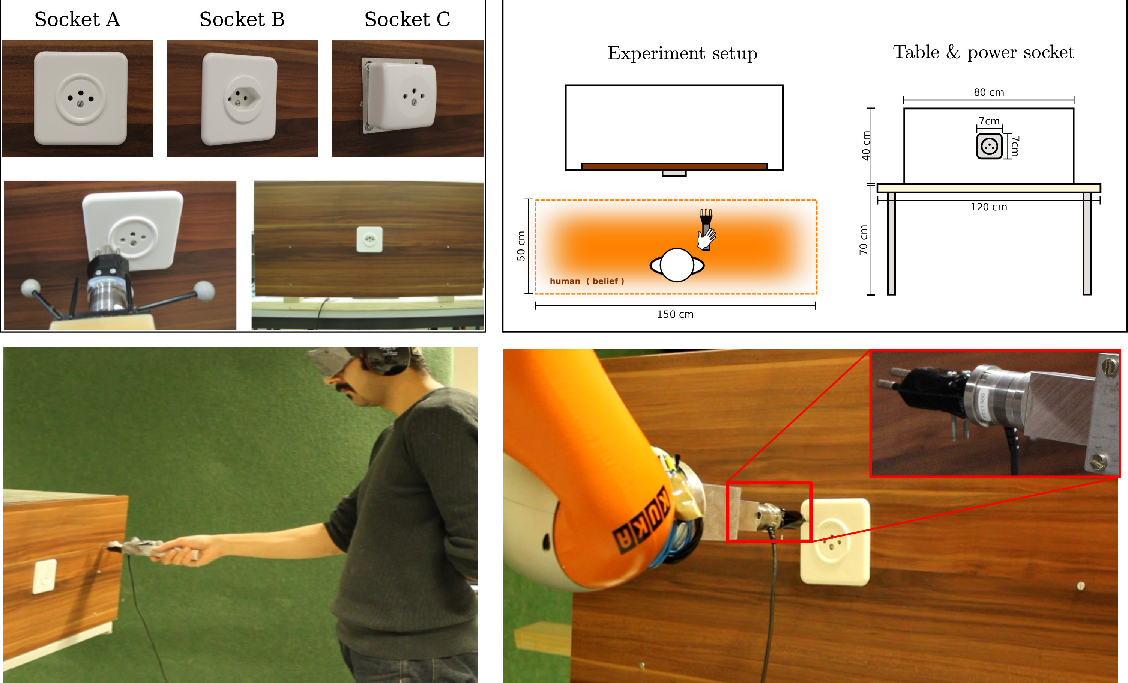
\includegraphics[width=0.85\linewidth]{./Figure/Figure1.pdf}
 \caption{\textbf{Peg-in-Hole search task setup}.
  \textit{Top-left}: Three different sockets are used, socket A will be only used to gather training data whilst socket B and 
  C will be used for evaluation purposes.  \textit{Top-right:} Dimensions of the the wall and socket, the orange area illustrates the possible locations 
  in which the human teacher will start the search.
  \textit{Bottom-left:} A participant (human teacher) is blindfolded and  placed within the orange rectangular area always 
  facing the wall. He is holding a cylinder equipped with a peg and an  ATI force torque sensor and OptiTrack markers. See \href{http://lasa.epfl.ch/videos/gpldecha/pih-search/human_search.wmv}{Video 1} for 
  an illustrate of a human subject performing the search task.
  \textit{Bottom-right:} The KUKA LWR robot is equipped with a peg holder mounted with an ATI force torque sensor, it is reproducing a search 
  and connection policy learned from the human demonstrations. See \href{http://lasa.epfl.ch/videos/gpldecha/pih-search/KUKA_pih-search.wmv}{Video 2} for an illustration of the KUKA searching for the socket and then 
  establishing a connection.}
    \label{fig:search_task_setup}
\end{figure*}

Figure \ref{fig:search_task_setup} (\textit{Top-right}), illustrates the PiH-search task. The orange area represents 
the teacher's starting area and is assumed prior knowledge. The sockets are always positioned at the center of a fake 
wall (wooden plank) which is clamped to a table. We consider one type of plug, 
Type J\footnote{http://www.iec.ch/worldplugs/typeJ.htm}, and three different power sockets. 
Power \textit{socket A}, has a ring around its holes, \textit{socket B} has a funnel, which we hypothesize should make 
it easier to connect, and \textit{socket C} has a flat elevated surface. See Figure \ref{fig:search_task_setup}
(\textit{Top-left}) for an illustration. 

To perform the PiH search tasks we recruited 10 student volunteers to be teachers (all male Master's and PhD students).
The participants were aged between 24 and 30 with an average age of 26 years and a standard deviation of 2.4 years.
Each participant carried out 30 demonstrations of the PiH search-task and each session lasted approximately 50 minutes and 
never exceeded one hour. The 10 participants were divided equally in two groups, A and B. Each member of group A began 
by performing 15 PiH searches with socket A (AA), followed by a 10 minute break, finishing with an additional 15 searches with socket B (AB). 
The members of group B performed the same protocol starting with socket B (BB) and ending with socket A (BA).
Figure \ref{fig:experiment_design} summarises a walk through of the experiment.
The only exclusion criteria was the inability of the subject to accomplish the task. All participants gave written consent 
for taking part in this study. A total of 300 demonstrations were gathered.

\begin{figure}
\centering
 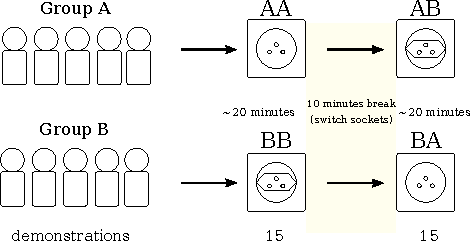
\includegraphics[width=0.9\linewidth]{./Figures/Fig/experiment_design_v2.pdf}
 \caption{Experiment protocol. The participants are divided in two groups of 5, Group A begins with socket A 
 and after a short break repeats the task with socket B. The same logic holds for Group B.
 For each socket 15 executions of the task are recorded.}
 \label{fig:experiment_design}
\end{figure}

\subsection{Data collection}

\begin{figure*}\label{fig:data-flow}
\centering
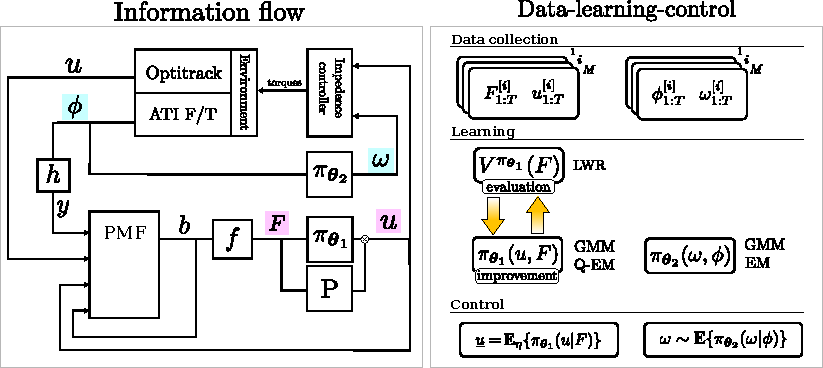
\includegraphics[width=0.9\linewidth]{./Figure/parameters-system-only-two-v2.pdf}
 \caption{\textit{Left:} The Point Mass Filter is updated with velocities, $u$ from the 
 Optitrack vision system when human demonstrations are being recorded. When the policy is active the PMF uses 
 the velocity output of policy $\pi_{\Param_1}$. The sensed wrench $\phi$ is transformed to a multivariate binary 
 feature vector which is used in the PMF state estimator. The filtered probability density, $b$ is compressed to a lower 
 dimensional feature vector $F$ before given as input to the linear velocity policy $\pi_{\Param_1}$. The second policy 
 $\pi_{\Param_2}$ outputs angular velocities $\omega$ given a sensed wrench $\phi$ and is used during the insertion stage of the PiH. 
 \textit{Right:} Data pipeline. First a set of $M$ demonstrates a dataset is created consisting of two subsets. Secondly, the left 
 dataset is used to learn policy $\pi_{\Param_1}$ in an Actor-Critic framework the dataset on the right is used 
 to directly learn the statistical policy $\pi_{\Param_2}$.}
\end{figure*}


The human teacher holds the plug which is attached to a cylindrical handle with 
an ATI 6 axis force torque sensor (Nano25 \footnote{http://www.ati-ia.com/products/ft/sensors.aspx}) 
to provide wrench $\phi \in \mathbb{R}^6$ measurements. We define measurement binary multivariate
feature to be a function of the wrench, $y = h(\phi)$. The feature vector encodes whether a contact is present 
and the direction in which it occurs, which is discretized to the four cardinalities.

On top of the cylinder there is a set of markers used by a motion capture system 
OptiTrack\footnote{http://www.optitrack.com/} (which has millimeter tracking accuracy) to measure 
both linear, $u \in \mathbb{R}^3$, and angular velocity, $\omega \in \mathbb{R}^3$, at each 
time step which is recorded at a rate of 100 Hz along with the F/T information. 


The location belief of the human teacher and robot apprentice is represented by a probability density function (pdf) ${b_t: = p(x_t|y_{0:t},u_{1:t})}$
which is represented by a Point Mass Filter (PMF) \cite[p.87]{Bergman99recursivebayesian}. PMF is chosen to represent the 
believed location of the plug as the sensing likelihoods are non-gaussian and lead to multi-modal distributions. 
Both $u$ and $y$ are used in the state transition and measurement model defined in the POMDP. Figure \ref{fig:PMF} (\textit{Left}) 
illustrates different time segments of the location belief recording during a demonstration. Figure \ref{fig:PMF} (\textit{Right}) illustrates 
the measurement likelihood function $\Omega := p(y_t|x_t)$ when an edge is sensed. 

As the belief is high dimensional it is impractical to directly learn a statistical policy ${\pi_{\theta} : b \rightarrow u }$ without 
some form of compression. We apply a compression function $f : b \mapsto F$ which transforms the belief to a lower 
dimensional feature vector  $F_t = [\hat{x}_t,U]^{\mathrm{T}}$ which for our purpose composed of 
the Most Likely State (MLS) $\hat{x}_t \in \mathbb{R}^3$ and differential entropy $U = H(b_t) \in \mathbb{R}$.

%which is assumed to be uniformly distributed in the orange area (refferece). All subsequent beliefs can be inferred from 
%the measured velocity and measurements provided by the ATI and OptiTrack sensors.

Each participant's demonstration results in a dataset ${D=\{u^{[i]}_{1:T},F^{[i]}_{1:T},\omega^{[i]}_{1:T},\phi^{[i]}_{1:T}\}}$, 
where the upper index $[i]$ references the ith search trajectory (one episode) and subscript $1:T$ denotes the time 
steps during the trajectory from initialisation $t=1$ until the end $t=T$. The information  flow is summarised in
Figure \ref{fig:data-flow} (\textit{Left}).

\begin{figure*}
 \centering
   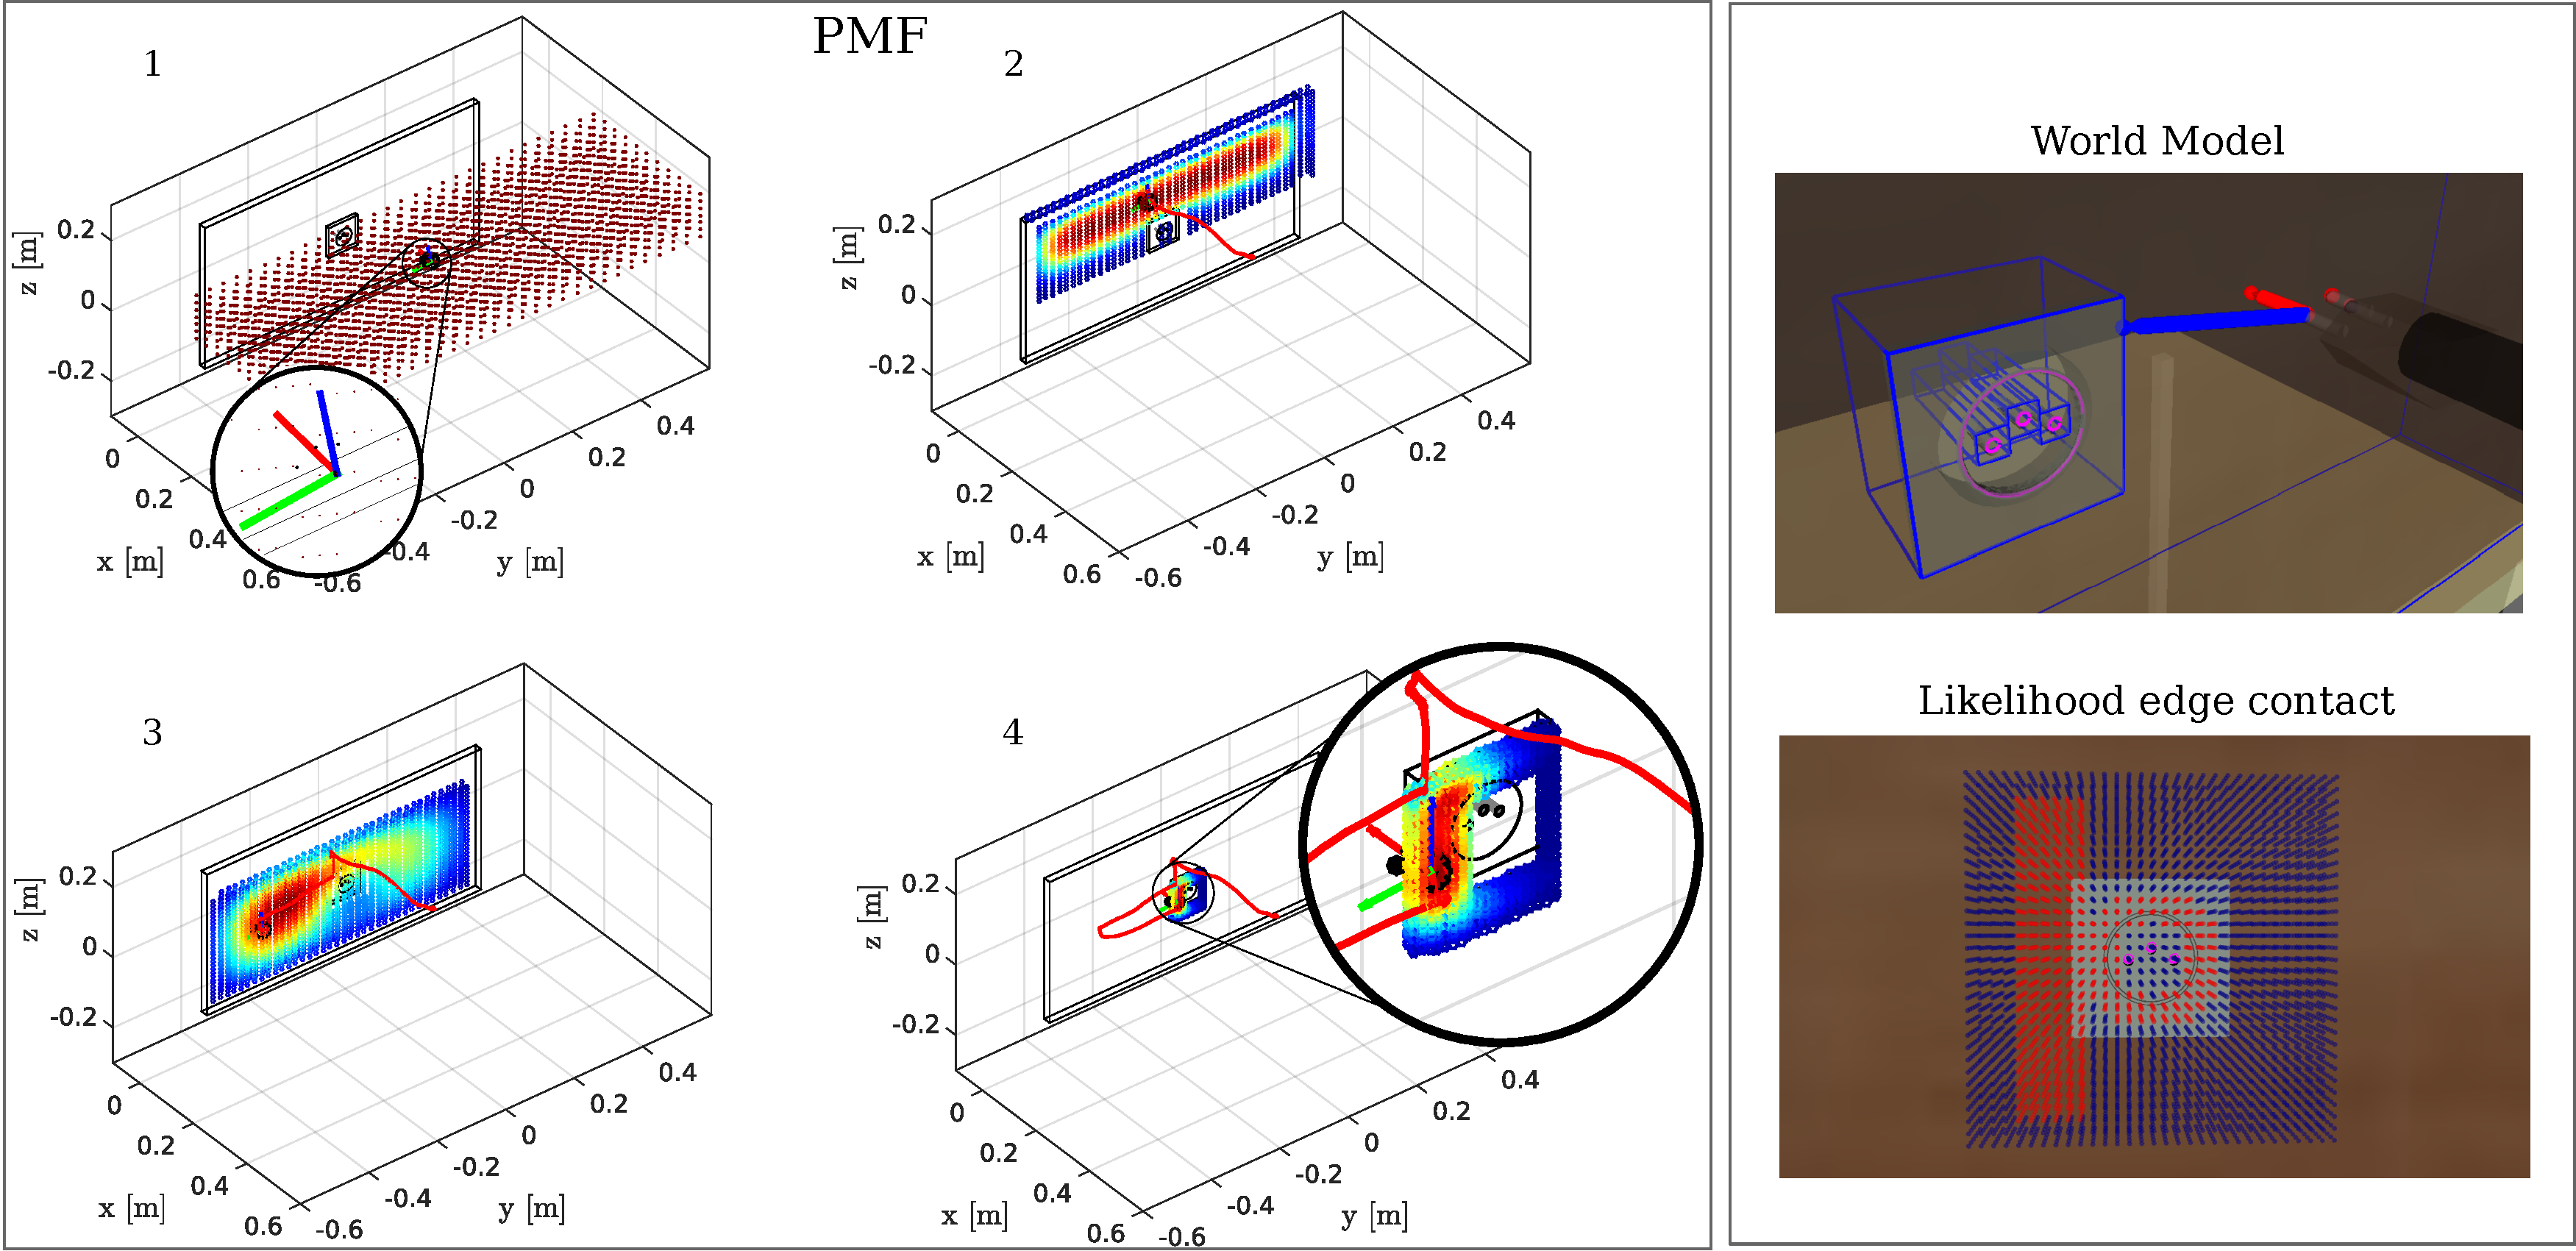
\includegraphics[width=0.95\textwidth]{./Figure/Figure2.pdf}
   \caption{\textit{Left:} Point Mass Filter (PMF) update of a particular human demonstration. (1) Initial uniform distribution spread over the starting 
   region. Each grid cell represents a hypothetical position of the plug. The orientation is assumed to be known. (2) First contact, the distribution 
   is spread across the surface of the wall. The red trace is the trajectory history. (3) motion noise increases the uncertainty. (4) The plug is in contact with a socket edge.
   See \href{http://lasa.epfl.ch/videos/gpldecha/pih-search/subject_PMF_belief_location.wmv}{Video 3} for an illustration of the PMF for a subject's search.
   \textit{Right}: \textbf{World model}: The plug is modelled by its three plug tips and the wall and sockets are fitted with bounding boxes.
   \textbf{Likelihood}: The plug enters in contact with the left edge of the socket. As a result, the value of the likelihood in all the regions, $x_t$, close the left edge take 
   a value of one (red points)  whilst the others have a value zero (blue points) and areas around the socket's central 
   ring have a value of one. }
  \label{fig:PMF}
\end{figure*}


\begin{figure}
 \centering
   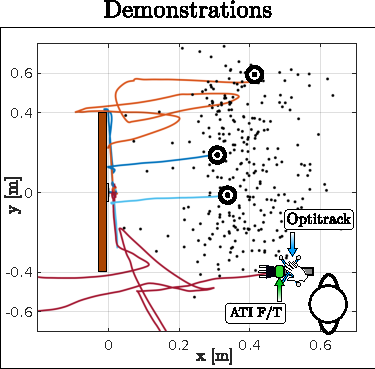
\includegraphics[width=0.9\linewidth]{./Figure/demonstrations.pdf}
   \caption{Black points represent the starting position of the end-effector
   for all the demonstrations. Four trajectories are illustrated.}
  \label{fig:experiment_setup_data}
\end{figure}

\section{Learning}\label{sec:learning-value-actor}

Two policies are learned: one maps a belief feature vector 
to linear velocity $\pi_{\Param_1} : F \mapsto u$ and the other to maps sensed wrench to angular 
velocity, $ \pi_{\Param_2} : \phi \mapsto \omega$.  Both linear and angular velocity policies are 
parameterised by a Gaussian Mixture Model (GMM), Equation \ref{eq:GMM}.

\begin{equation}
 \pi_{\Param}(\xi_1,\xi_2) = \sum\limits_{k=1}^{K} \piK \, g(\xi_1,\xi_2;\MuK,\SigK) \label{eq:GMM}
\end{equation}
The parameters $\Param = \{w^{[k]},\MuK,\SigK\}_{1,\dots,K}$, are the weights, means and covariances 
of the individual Gaussian functions $g(\cdot)$
\begin{center}
$\MuK =  \begin{bmatrix} \MuK_{\xi_1} \\ \MuK_{\xi_2} \end{bmatrix}$\hspace*{0.5cm}
$\SigK =  \begin{bmatrix} 
	  \SigK_{\xi_1\xi_1} & \SigK_{\xi_1\xi_2} \\
	  \SigK_{\xi_2\xi_1} & \SigK_{\xi_2\xi_2}
	  \end{bmatrix}$
\end{center}
and $\sum_{k} w^{[k]} = 1$. For the linear policy policy $\pi_{\Param_1}$: ${\xi_1 = u}$ and ${\xi_2 = F}$.
For the angular policy $\pi_{\Param_2}$: ${\xi_1 = \omega}$ and ${\xi_2 = \phi}$. In both cases the Bayesian Information Criterion is used to 
determine the number of Gaussian functions.

The parameters of the linear velocity policy $\pi_{\Param_1}$ are learned in our Fitted Policy Iteration framework
whilst the parameters of the angular velocity policy $\pi_{\Param_2}$ are directly learned from the demonstrations following 
the methodology outlined in \cite[Chap. 5]{Kronander2015}. 
%This proves to be efficient in overcoming jamming during the final insertion step of PiH. 

\subsection{Fitted Policy Iteration}\label{sec:FPI}

Policy Iteration is an on-policy off-line reinforcement learning method which through successive iterations of policy \textit{evaluation} 
and \textit{improvement} both value function and policy converge to their optimal parameters \cite[Chap. 4.6]{sutton1998reinforcement}.

\paragraph{Policy evaluation}
%s and then policy is maximised it with respect to its parameters.
%In an Actor-Critic setting, the temporal difference error, ${\delta^{\pi}_t = r_{t+1} + \gamma \hat{V}^{\pi}(F_{t+1}) - \hat{V}^{\pi}(F_t)}$, 
%of the value function is used as a learning signal to update simultaneously itself and the actor.

A value function, Equation \ref{eq:value_function}, of the belief state feature vector $F$ is  learned from the 
trajectory data provided by the teachers.

\begin{equation}\label{eq:value_function}
  V^{\pi_{\Param_1}}(F) = \mathbb{E}_{\pi_{\Param_1}}\Bigg\{  \sum^{\infty}_{k=0} \gamma^k r_{t+k+1} \Bigg\lvert  F_t=F\Bigg\}
\end{equation}

A reward of ${r=0}$ is assigned at each time step until the goal (plug-socket connection) is achieved, where a 
reward of $r_{T}=100$ is obtained. Given the continuous nature of the belief feature vector Locally Weighted Regression
(LWR) \cite{Atkeson97locallyweighted}  is used as a function approximator of the value function.

To learn the value function Fitted/Batch RL approach is taken\cite{EGW05}, an offline method which applies multiple 
sweeps of the Bellman backup operator followed by fitting the value function through regression to a dataset of 
tuples $\{(F^{[i]}_t,r^{[i]}_t,F^{[i]}_{t+1})\}_{i=1,\cdots,M}$ until the Bellman residual 
converges, see Algorithm \ref{alg:fpe}.

\begin{center}
\begin{minipage}{\linewidth}
\removelatexerror% Nullify \@latex@error
\begin{algorithm*}[H]
\label{alg:fpe}
\SetKwInOut{Input}{input}
\SetKwInOut{Output}{output}
\Input{$\epsilon$, $\{(F^{[i]}_t,r^{[i]},F^{[i]}_{t+1})\}_{i=1,\cdots,M}$}
\Output{$\hat{V}^{\pi}_{k}(F)$}
\BlankLine
\While{$||\hat{V}^{\pi}_{k+1}(\B) - \hat{V}^{\pi}_{k}(\B)|| > \epsilon$}{
  $\hat{V}^{\pi}_{k+1}(F)$ = Regress($F_t$, $r_t + \gamma \hat{V}^{\pi}_k(F_{t+1}))$
}
\caption{Fitted Policy Evaluation}
\end{algorithm*} 
\end{minipage}
\end{center}

Most Fitted RL methods have focused on learning the Q-value function directly (Fitted Q-Iteration) 
\cite{NIPS2008_3501,EGW05,Riedmiller2005}. Although this solves the control problem it requires discretisation 
of the action space or assumes quantifiable actions, so that maximisation in the Q-Bellman backup
${\max_{u_{t+1}} \hat{Q}(u_{t+1},F_{t+1})}$ is easily achievable. Given the dimensionality and continuity 
of our problem we assume this to be unrealistic and we opt for a fitted .

\paragraph{Policy improvement}

The actor is updated given the critic's value function through a modification of the Maximisation step in  Expectation-Maximisation (EM) 
for Gaussian Mixture Models. This modification is referred to as Q-EM which is strongly related to a Monte-Carlo EM-based policy 
search approach \cite[p.50]{p_search_surv_2011}. 

The reward of a demonstrated trajectory (one episode) is given by the sum of discounted return, Equation $\ref{eq:disc_return}$,
\begin{equation}\label{eq:disc_return}
 R_T(e_i) = \sum_{t=0}^{\mathrm{T^{[i]}}} \gamma^t \, r(u^{[i]}_t,F^{[i]}_t)
\end{equation}
where $e_i = \{(u_0,F_0),\cdots,(u_T^{[i]},F_T^{[i]}) \}$ are the state-action samples of the $ith$ episode.
All policy gradient approaches seek to find a set of parameters $\Param$ of the actor,
which will maximise the expected reward, Equation \ref{eq:expected_reward},

\begin{equation}\label{eq:expected_reward}
 J(\Param) = \mathbb{E}_{p_{\Param}}\{R_T\} = \sum\limits_{i=1}^{N}
 \underbrace{\left( \prod_{t=0}^{T^{[i]}} \pi_{\Param}(u^{[i]}_t,F^{[i]}_t) \right)}_{p_{\Param}(e_i)} \, R_T(e_i) 
\end{equation}

By setting the derivative to zero, the parameters which maximise the cost function $\argmax_{\Param} J(\Param)$
can be found. This cannot be done directly, instead the logarithmic lower bound of the cost function is maximised which results in 
Equation \ref{eq:grad_log_cost}. See \cite[p.50]{p_search_surv_2011} for the derivation. 

\begin{equation} \label{eq:grad_log_cost}
  \nabla_{\Param}\mathcal{Q}(\Param,\Param') = \sum\limits_{i=1}^{N} \sum\limits_{t=0}^{T^{[i]}} \nabla_{\Param}\log \pi_{\Param}(u^{[i]}_t,F^{[i]}_t) \, Q^{\pi_{\Param'}}(u^{[i]}_t,F^{[i]}_t)
\end{equation}
In the above equation $\Param'$ are the parameters used to generate the trajectories during the E-step. In our case these are 
the initial demonstrations provided by the teachers.
In most policy search approaches the policy is conditioned on the state space, $\pi_{\Param}(\U_t|\B_t)$. This would lead
to a complex expression in the maximisation of Equation \ref{eq:grad_log_cost} and is restrictive in the case of the GMM as it 
fixes the state space parameters $\MuK_{F}$, $\SigK_{FF}$ (and partially $\SigK_{uF}$) and thus greatly constrains the solution.
Instead Equation \ref{eq:grad_log_cost} is optimised with respect to the joint distribution $\pi_{\Param}(u,F)$ and not 
the conditional $\pi_{\Param}(u|F)$. This has two benefits. Firstly, the input dimensions (the state space) are no 
longer fixed allowing the GMM basis functions to move and secondly the optimisation of GMM parameters is very similar to 
that of the traditional EM. Setting the derivative of Equation \ref{eq:grad_log_cost} to zero and solving for the parameters
$\Param=\{w,\boldsymbol{\mu},\boldsymbol{\Sigma}\}$ a new weighted (by $Q^{\pi_{\Param'}}$) Maximisation EM step, 
see Figure \ref{fig:Q-EM}, is obtained.

\begin{figure}\label{fig:Q-EM}
\begin{empheq}[box={\tcbhighmath[colback=blue!2,colframe=blue]}]{align}
    \MuK_{\textrm{\textbf{new}}}    &= \frac{\sum\limits_{j=1}^{M} \alpha_k(\Bx^{[j]})\, \Qpx \, \Bx^{[j]} }{\sum\limits_{j=1}^{M} \alpha_k(\Bx^{[j]})\, \Qpx} \nonumber \\
    & \nonumber\\
    \SigK_{\textrm{\textbf{new}}}   &= \frac{\sum\limits_{j=1}^{M}  \alpha_k(\Bx^{[j]})\, \Qpx (\Bx^{[j]} - \MuK_{\textrm{\textbf{new}}}  )(\Bx^{[j]} - \MuK_{\textrm{\textbf{new}}}  )^{\mathrm{T}} }{ \sum\limits_{j=1}^{M} \alpha_k(\Bx^{[j]})\, \Qpx } \nonumber  \\
    & \nonumber\\
    w^{[k]}_{\textrm{\textbf{new}}} &= \frac{\sum\limits_{j=1}^{M} \Qpx \, \alpha_k(\Bx^{[j]})}{\sum\limits_{j=1}^{M} \Qpx} \nonumber
\end{empheq}
\caption{Q-EM Maximisation of the GMM parameters. We used the same notation and derivation as in \cite[Chap. 9.2.2]{Bishop_2006}, where $\alpha_k(\Bx^{[j]})$ is 
the responsibility factor, denoting the probability that data point $\mathbf{x}^{[j]} = [u^{[j]},F^{[j]}]^{\mathrm{T}}$ belongs to  Gaussian function $k$.}
\end{figure}

As for the learned value function in the policy evaluation step, the advantage function
\begin{equation}\label{eq:advantage_f}
 A^{\pi_{\Param}}(u_t,F_t) =  Q^{\pi_{\Param}}(u_t,F_t) - V^{\pi_{\Param}}(F_t) = \delta^{\pi_{\Param}}_t
\end{equation}
is used as a substitute for $Q^{\pi}$ which is derived from the TD error. Assuming that the estimated 
value function, $\hat{V}^{\pi}$, is close to the true value function $V^{\pi}$, the 
TD error $\delta^{\pi}$ is an unbiased estimate of the advantage function. Using the 
advantage function as means of policy search is popular with methods such as Natural Actor Critic (NAC) \cite{peter_nac_2008}.

Each state-action sample $j$ has an associated weight, $\delta_j \in \mathbb{R}$, where $\delta_j > 0$ means that the 
$j$th state action-pair lead to an increase in the value function and $\delta_j < 0$ lead to 
a decrease in the value function. The data log-likelihood is re-weighted accordingly, giving more importance to data points which lead to a gain. Since 
the Q-EM update steps cannot allow negative weights, the TD error is rescaled to be between 0 and 1. 


\paragraph{2D example fitted policy iteration}

To illustrate the mechanism of fitted policy iteration, we give a 2D example 
of its application, see Figure \ref{fig:fpe_example}. The \textit{Top-left} subfigure
depicts 10 trajectories demonstrated by two teachers going from start (white circle) to goal (orange star) state. 
The optimal path is a straight line passing in between two obstacles. 
Neither teacher demonstrated the optimal straight path. 

In the \textit{Bottom-left}, a GMM is fitted $\pi_{\Param}(\U,\X)$ to the teachers' data, using the standard EM-algorithm.
Taking the policy to be the output of Gaussian Mixture Regression (GMR) $\mathbb{E}\{\pi_{\Param}(\U|\X)\}$ different
behaviours are obtained than those demonstrated by the human teachers. The GMR averages the different modes encoded by the Gaussian functions 
which results in a mixing of the original demonstrated behaviours. No trajectories of the GMR policy truly replicate 
the demonstrated behaviour. 

In the \textit{Top-right} subfigure, we apply fitted policy evaluation to the original demonstrated data (discount 
factor $\gamma=0.99$ and reward $r_{T}=1$ when the goal is reached and zero otherwise) and compute the value function.

The \textit{Bottom-right} subfigure illustrates the GMM policy learned with the Q-EM algorithm. As 
the advantage function $ A^{\pi}(\X,\U)$ is highest along the start-goal axis, data points
following this gradient will have a higher weight. This results in a policy with better 
rollouts (closer to the optimal path) than the trajectories generated by the policy learned via standard EM. 

\begin{figure}
 \centering
 \setlength\fboxsep{0pt}
  \setlength\fboxrule{0.25pt}
  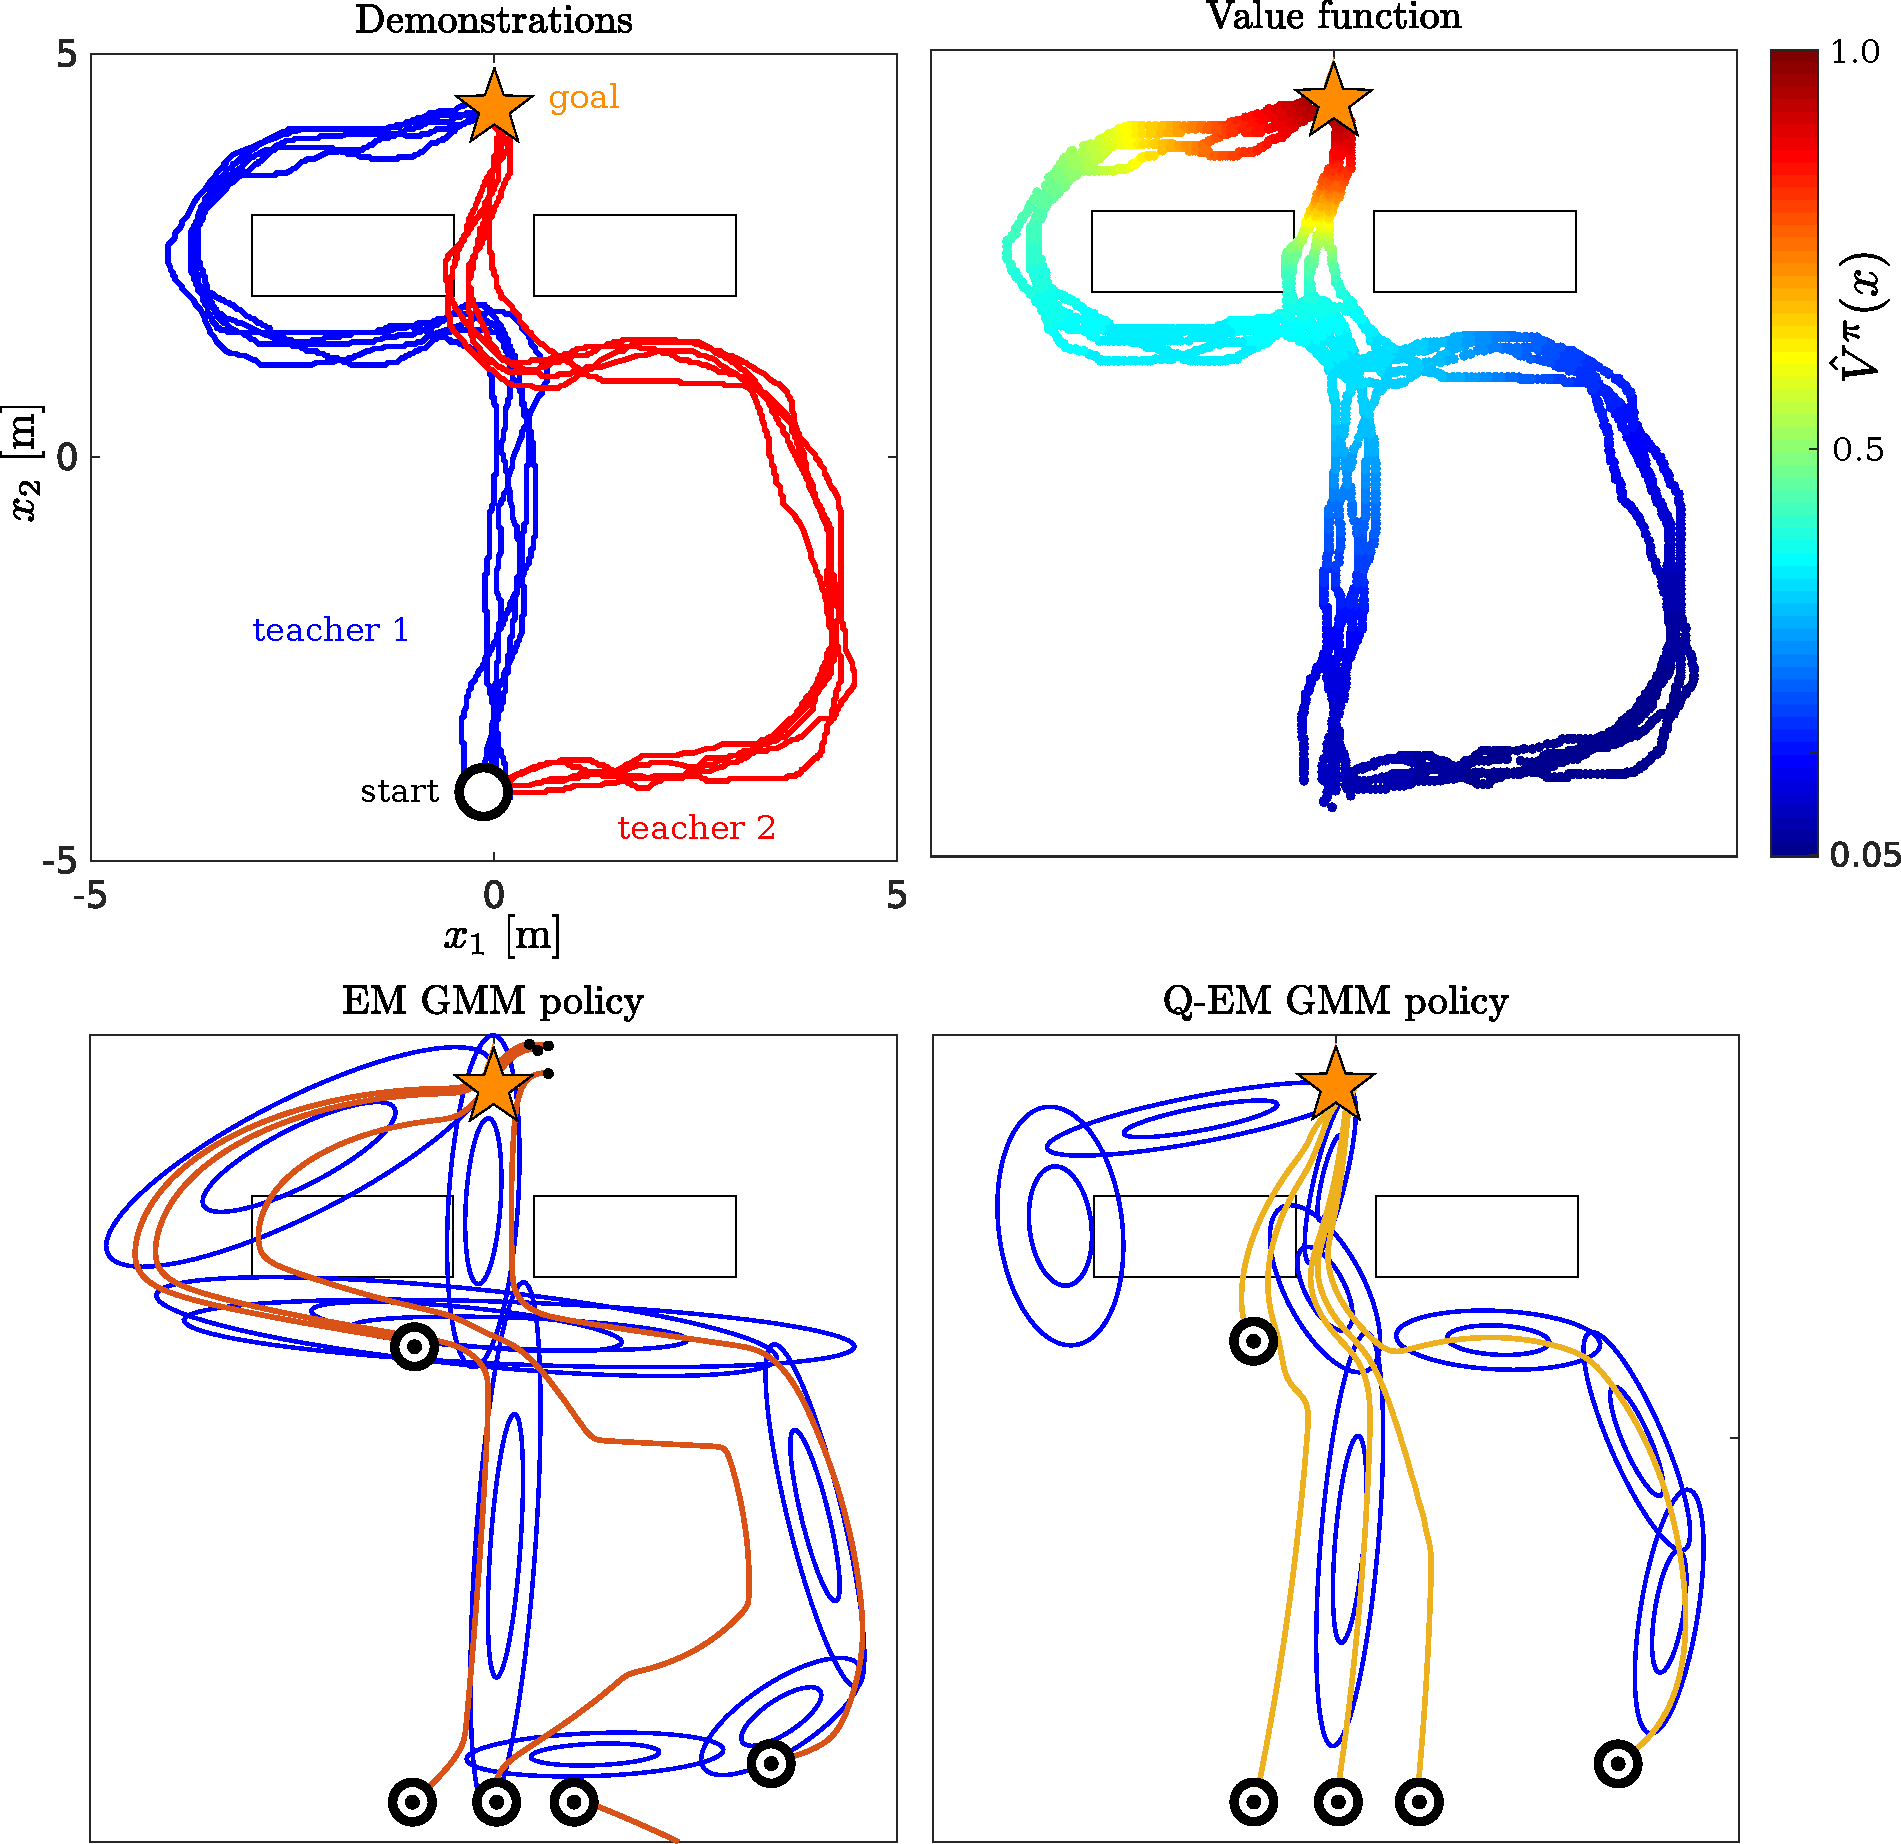
\includegraphics[width=\linewidth]{./Figure/fpe_example.pdf}
 \caption{Fitted policy evaluation \& improvement example. 
  \textit{Top-left:} The goal of the task is to reach the goal state. The first teacher (blue) demonstrates 
  five trajectories which contour the obstacle in front of the goal. The second teacher (red) demonstrates 
  5 trajectories which initially deviate from the goal before passing between the two obstacles. 
  \textit{Bottom-left:} The EM algorithm is used to fit a GMM to the teachers' original data. 
  The marginal $\pi_{\Param}(\X)$ is plotted in blue and trajectories generated by the 
  policy $\mathbb{E}\{\pi_{\Param}(\U|\X)\}$ in orange. \textit{Top-right} \textit{Policy Evaluation:}.  
  Value function after fitted policy evaluation terminated, the reward function 
  is binary, $r_T=1$ at the goal and zero otherwise, and a discount factor $\gamma = 0.99$ is used.
  \textit{Bottom-right} \textit{Policy Improvement:} the GMM is learned with the Q-EM algorithm in which 
  each data point's weight is proportional to the advantage function.
 }
  \label{fig:fpe_example}
\end{figure}

\paragraph{Belief state fitted policy evaluation}

FPI is applied to the data from demonstrations done on socket A. Figure \ref{fig:ch4:Figure1} (\textit{Left}) illustrates 
the value function of the most likely state. As expected, the value function is high closest to the socket and around the axis $z=0$ and $y=0$. 
When Q-EM is applied the Gaussian functions of the GMM will favour these locations. 

\begin{figure*}
 \centering
 
\includegraphics[width=\linewidth]{./Figure/value_function_belief.pdf}
 \caption{\textit{Left}: LWR value function approximate $\hat{V}^{\pi}(\hat{x})$ for the most likely state $\hat{x}$. 
 The red plane is to help visualise where the value function is above and below the axis $z=0$. Only states with values above
 $0.25$ are plotted.  The red arrow indicates the heading of the human teacher when performing the search task. The discount 
 factor was $\gamma=0.99$ and the variance of the kernel variance of 1 [cm], which was set experimentally.
 \textit{Middle-right}: Best and worst trajectories. The red demonstrated trajectories are the best in terms of the amount of value function 
 gain whilst the blue are the worst. The red arrow indicates the teacher's heading. The blue trajectories tend 
 towards the sides of the wall as the initial starting position is on the border of the wall. The red trajectories are centred along the y-axis of socket and tend to move in a straight line towards 
 the wall whilst aligning themselves with the axis $z=0$.
}
 \label{fig:ch4:Figure1}
\end{figure*}

Figure \ref{fig:ch4:Figure1} (\textit{Middle}-right) illustrates the best and worst trajectories in terms of the accumulated value function.
It can be seen that the best trajectories (red) tend to be aligned with the socket (star position in front of socket), 
whilst the worst trajectories are towards the edges of the wall and tend to follow spiralling motions. 

In conclusion we learned two policies, one solely from the original human demonstrations which we call GMM and the second which 
is the result of \textbf{one iteration} of fitted policy iteration which we call Q-EM. This compares the effect
of one policy evaluation and improvement sequence have without doing any additional rollouts. This ensures that both policies
are given the same amount of information.

\section{Control architecture}\label{sec:control_architecture}

The direction to search is given by the conditional:

\begin{equation}\label{eq:gmm_conditional}
 \pi_{\Param_1}(u\lvert F) = \sum_{k=1}^{K} w^{[k]}_{\xb} \; g(u;\MuK_{\xb},\SigK_{\xb}) 
 \end{equation}

which is a distribution over the possible normalised velocities. The function $g(\cdot)$ is a multivariate
Gaussian function parameterised by mean $\MuK_{\xb} \in \mathbb{R}^{(3\times1)}$ and Covariance $\SigK_{\xb} \in \mathbb{R}^{(3\times3)}$. The subscript $\xb$ indicates that the parameters 
are the result of the conditional. The reader is referred to \cite{gesture_calinon_2010}, \cite{gmr_2004} for 
a detailed derivation of the conditional of a GMM. The learned model 
is multi-modal, as different search velocities are possible 
in the same belief state. Figure \ref{fig:policy_vf} illustrates the multi-modal 
vector fields of the conditional, Equation \ref{eq:gmm_conditional}.
In autonomous dynamical systems control, the velocity is obtained from 
the expectation of the conditional, Equation \ref{eq:gmm_conditional}. However, the expectation which is a weighted 
linear combination of the modes, could result in unobserved behaviour or no movement if the velocities cancel out. 
As a result we use a modified version of the expectation operator which favours the current
direction, Equation \ref{eq:alpha_eq} - \ref{eq:alpha_expectation}.

\begin{align}
 \eta_k(u) &= w^{[k]}_{\xb} \cdot \exp(-\cos^{-1}(<u,\MuK_{\xb}>)) \label{eq:alpha_eq}\\
 \underline{u} &= \mathbb{E}_{\eta}\{\pi_{\Param}(\xb)\} = \sum_{k=1}^K \eta_k(u) \cdot \MuK_{\xb} \label{eq:alpha_expectation}
\end{align}
The GMM policy $\underbar{u} = \mathbb{E}_{\eta}\{\pi_{\Param}(u \lvert F)\}$ outputs a linear velocity which 
is normalised, $\underbar{u} \in \mathbb{R}^{(3 \times 1)}$. When the applied velocity mode is no longer present another direction is sampled. 
For example, when the robot enters in contact with a feature, greatly reducing the uncertainty, the current mode changes and a new search direction is computed. 
Figure \ref{fig:policy_vf} illustrates the policy vector field for GMM and Q-EM, both learned from teachers demonstrations.

\begin{figure}
   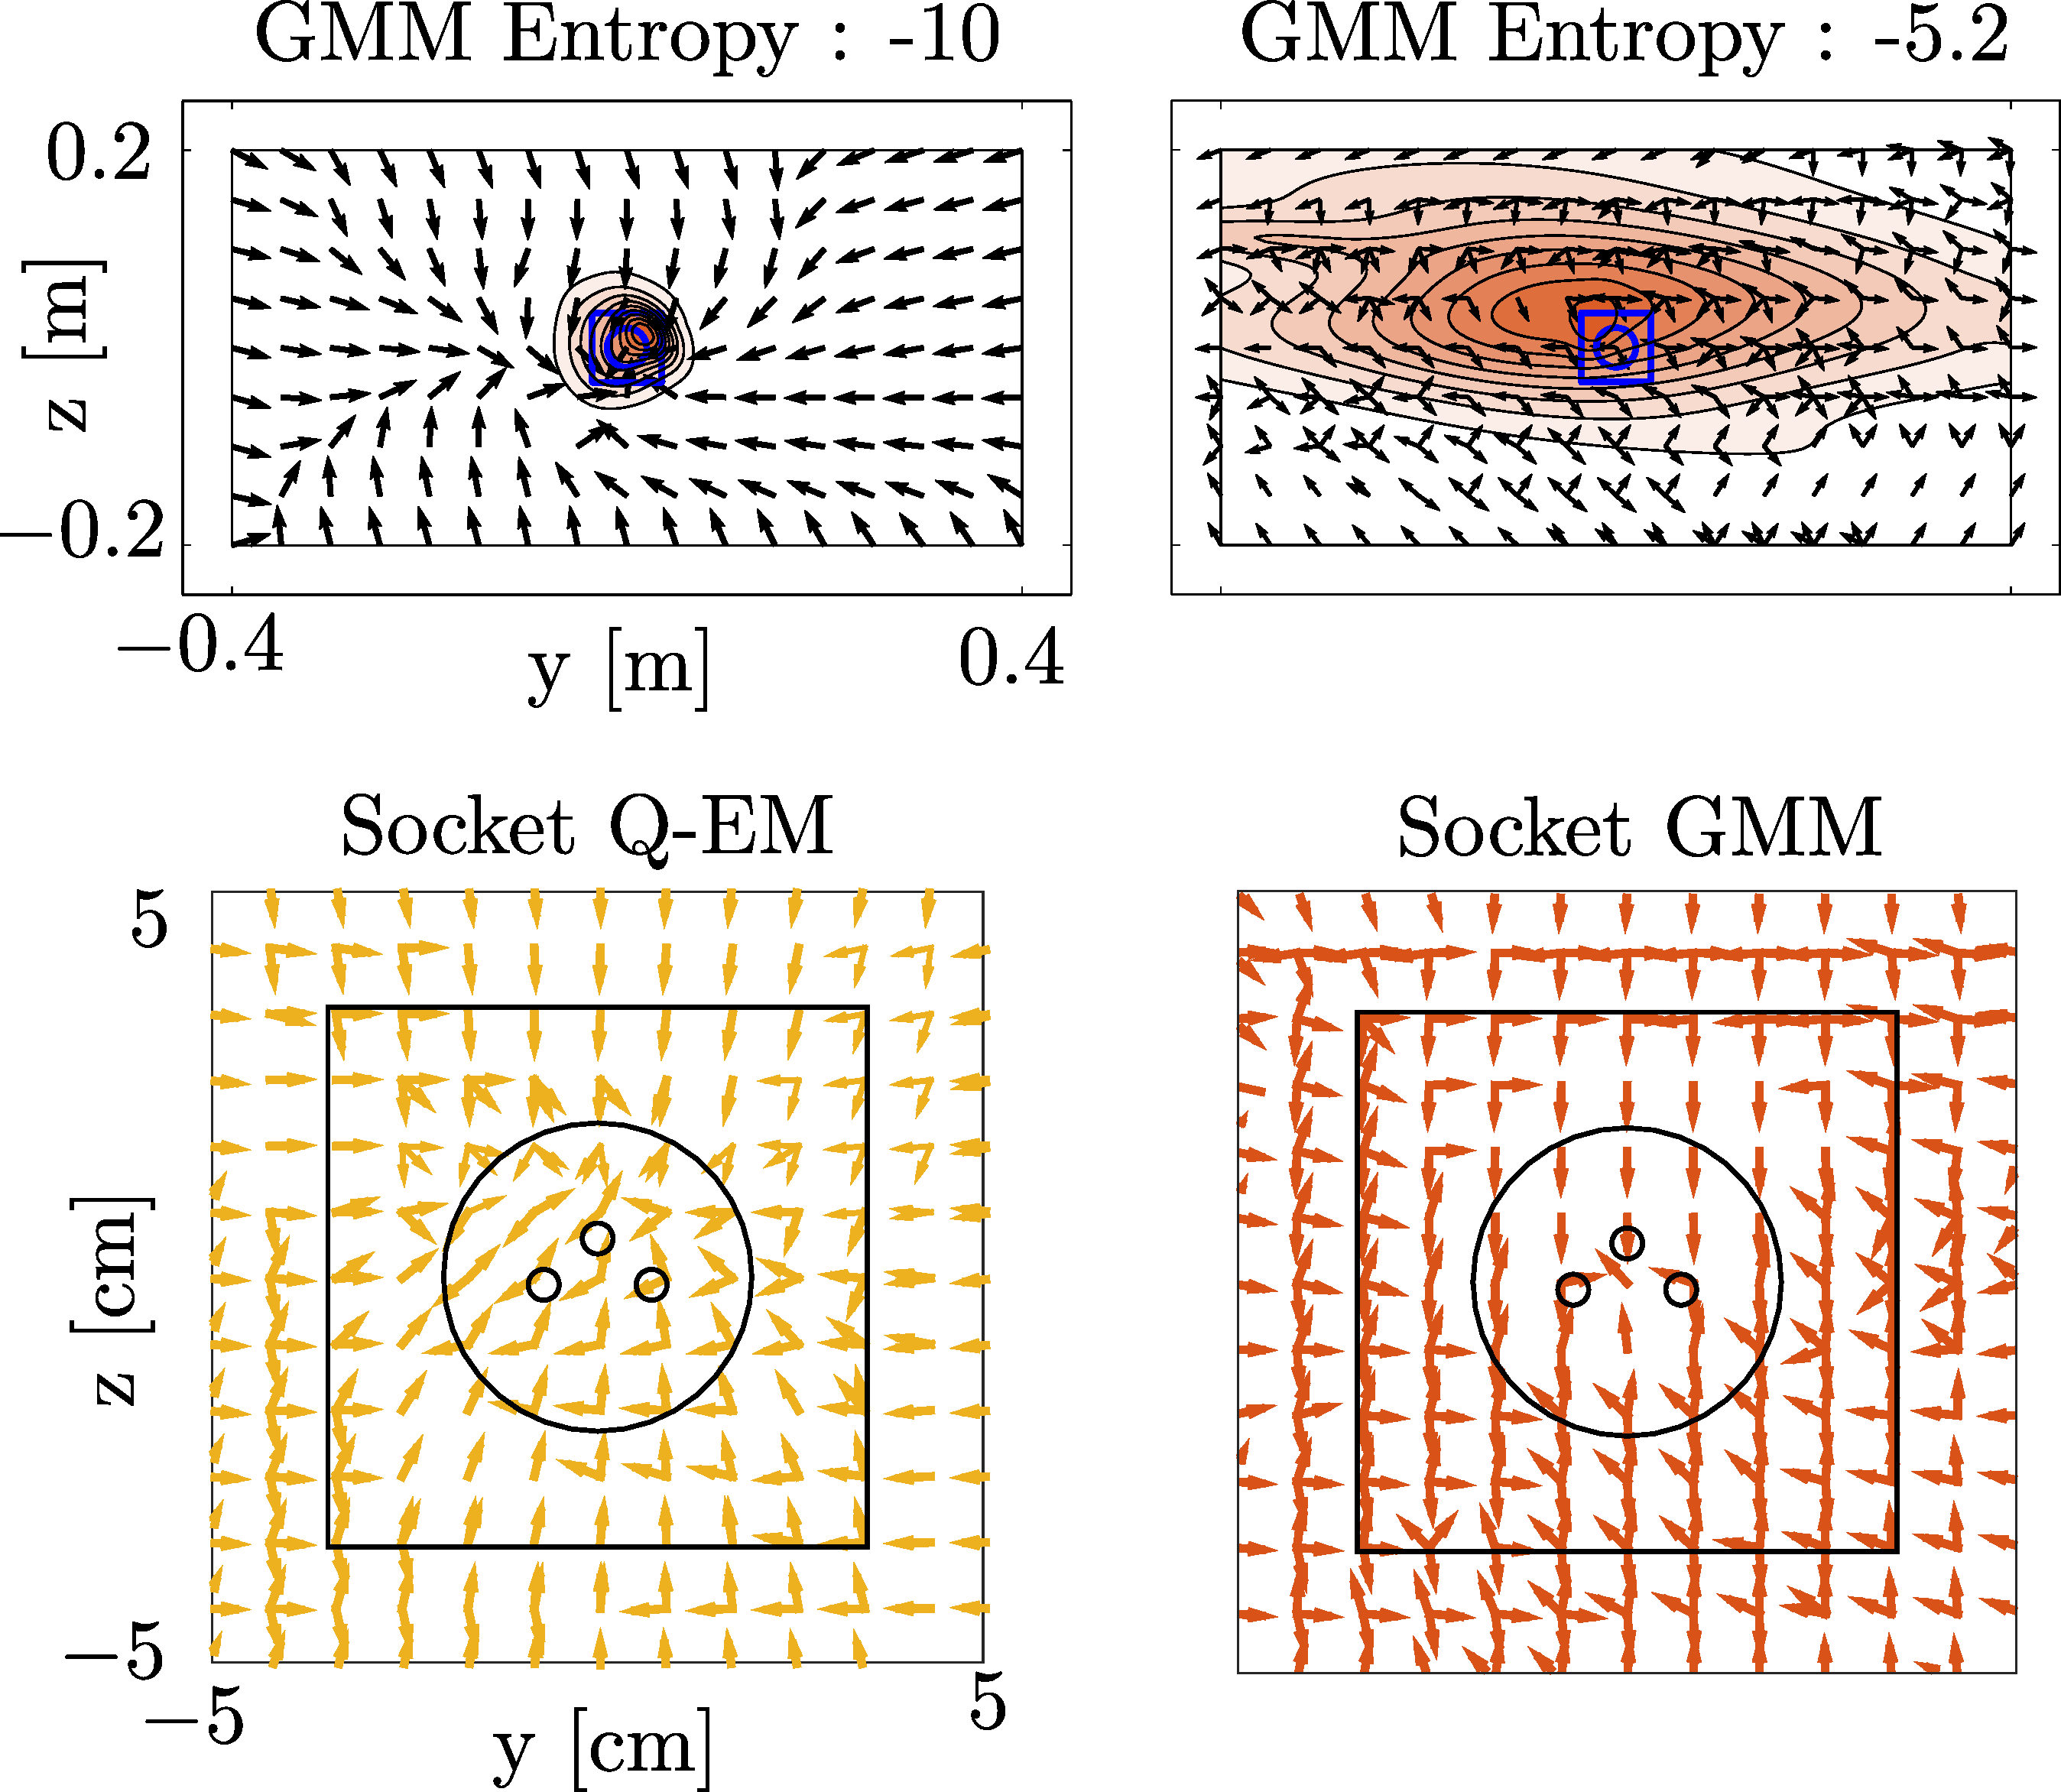
\includegraphics[width=0.45\textwidth]{./Figures/Fig/policy_vf.pdf}
  \caption{Q-EM and GMM policy vector fields. \textit{Top}: The GMM policy is conditioned on an entropy of $-10$ and $-5.2$. For the lowest entropy level,
  most of the probability mass is close to the socket area since this level corresponds to very little uncertainty; we are already localised. We can see 
  that the policy converges to the socket area regardless of the location of the believed state. For an entropy of $-5.2$ we can see that 
  the likelihood of the policy is present across wall. The vector field directs the end-effector to go towards the left or right edge of the wall. 
  \textit{Bottom}: The entropy is marginalised out, the yellow vector field is of the Q-EM and orange of the GMM. The Q-EM vector field tends 
  to be closer to a sink and there is less variation.}
  \label{fig:policy_vf}
\end{figure}

\subsection{Robot Implementation}


This search task is haptic and the end-effector of the robot is always in contact with the environment. To make the robot
compliant with the environment we use an impedance controller in combination with a hybrid position-force controller. The hybrid controller
targets a sensed force $F_x$, in the $x$-axis, of 3N. The $y$ and $z$ velocity components of the direction vector are given by 
Equation \ref{eq:alpha_expectation}. This is insufficient for the robot to reliably surmount the edges of the socket,
hence the vector field of the GMM is modulated in $y$ and $z$-axis, Equation \ref{eq:modulation}.

\begin{equation}
  \underbar{u} = R_y(c(F_z) \cdot \pi/2) \cdot R_z(c(F_y) \cdot \pi/2) \cdot \underbar{u} \label{eq:modulation}
\end{equation}

where $R_y$ and $R_z$ are $(3 \times 3)$ rotation matrices around the $y$ and $z$-axis, and $c(force) \in [-1,1]$ is a truncated scaling function of the sensed 
force.  When a force $F_z$ of 5N is sensed, a rotation of $R_y(\pi/2)$ is applied to the original direction resulting in the robot
getting over the edge. The direction velocity is always normalised up to this point. The amplitude of the velocity is a proportional
controller based on the believed distance to the goal. 
%Figure \ref{fig:control_flow} illustrates the complete control flow.
%\begin{figure}
%  \centering
%  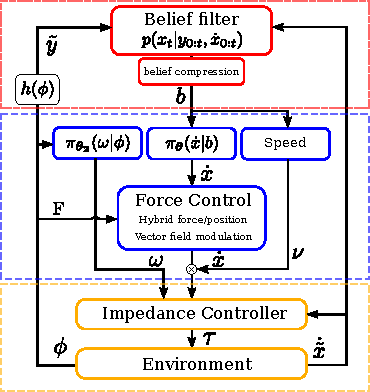
\includegraphics[width=0.45\textwidth]{./Figures/control_flow_final.pdf}
%  \caption{Control architecture. The PMF (belief) receives a measured velocity, $\dot{\tilde{x}}$, and 
%  a sensor measurement $\tilde{y}$ and is updated via Bayes rule. The belief is compressed and used by 
%  both the GMM policy and the proportional speed controller.}
%  \label{fig:control_flow}
%\end{figure}

\section{Results}\label{sec:results}

We evaluate the following three aspects:
\begin{enumerate}
 \item \textbf{Distance taken to accomplish the goal} (connect plug to socket). We compare the Q-EM policy with 
 a GMM policy learned through standard EM and a myopic Greedy policy. This highlights the difference between complicated and simplistic  
  search algorithms and gives an appreciation of the problem's difficulty.
 \item \textbf{Importance of data} provided by human teachers. We evaluate whether it is possible to learn 
 an improved GMM policy from Greedy demonstrations. This policy which we call Q-Greedy is used to test whether 
 indeed human demonstrations are necessary. We evaluate whether it is possible to obtain a good policy from the two worst teachers' demonstrations as not all teachers 
 are necessarily proficient at the task in question. 
  \item \textbf{Generalisation}. We learn a policy to insert a plug into socket A which is located at the center of a wooden 
 wall. We test the generalisation of the policy in finding a new socket location and whether the policy can generalise to sockets 
 B and C, which were not used during the training phase.
\end{enumerate}

We evaluate aspects 1) and 2) purely in simulation as finding the socket requires much less precision than establishing a 
connection and the physics of the interaction is simple. Aspect 3), the generalisation, is evaluated both in simulation,
up to the point of localising the socket's edge, and on the KUKA LWR robotic platform
for the connection phase of the task. The main reason for employing the robot is that the connection phase dynamics is 
complex and a simulation would be unrealistic. For the robot evaluation we consider 
the search starting already within the vicinity of the socket.

\subsection{Distance taken to reach the socket's edge}

We consider two search experiments which we refer to as \textbf{Experiment 1} and \textbf{2}, in order to evaluate the performance 
in terms of the distance travelled to reach the socket for the three search policies: GMM, Q-EM and Greedy. In these two 
experiments the task is considered accomplished when a search policy finds the socket's edge. 

\textbf{Experiment 1}, three starting locations are chosen: \textit{Center}, \textit{Left} and \textit{Right}. 
See Figure \ref{fig:experiment12} \textit{(Experiment 1 Top-left)}, for an illustration of the initial condition. 
This setup tests the effect of the starting positions. A total of 25 searches are carried out for each of the search policies.
The trajectory results show a clear difference between the trajectories generated by the GMM and Q-EM policies (\textit{Experiment 1 Bottom-left}). 
The orange GMM policy trajectories go straight towards the wall, whilst the yellow Q-EM policy trajectories drop in height 
making them closer to the socket. 
\textit{Experiment 1 Bottom-right}, illustrates the distribution of the first contact with the wall for the \textit{Center} initial 
condition. The distribution of the first contact of the Greedy method is uniform across the entire $y$-axis of the wall. 
It does not take into account the variance of the uncertainty. In contrast, the GMM policy remains centred 
with respect to the starting position and the Q-EM is even closer to the socket and there is much less variance in 
the location of the first contact.

\textit{Experiment 1 Top-right}, illustrates the quantitative results of the distance taken to reach the socket for 
all three experiments. For the \textit{Center} initial condition, the Q-EM policy travels far less than the other search policies. 
Considering that the initial position of the search is 0.45 [m] away from the wall, the Q-EM policy finds the socket very 
quickly once contact has been established with the wall. For the \textit{Right} and \textit{Left} starting conditions both 
the GMM and Q-EM policies travel less distance to reach the socket, with a smaller variance when compared with the Greedy search policy.

\textbf{Experiment 2}, Figure \ref{fig:experiment12} (\textit{Experiment 2}), the initial true starting positions 
of the end-effector are taken from a regular grid, within the red cube (see \textit{Experiment 1}), covering the whole start region, also used as the initial distribution for 
the human demonstrations. A total of a 150 searches are carried out for each of the three policies. 
This experiment compares the search policies with the human teachers' demonstrations. 
The Human and GMM show similar distributions of searched locations. They cover the upper region of the wall and top corners, to some extent. These distributions 
are not identical for two reasons. The first is that the learning of the GMM is a local optimisation 
which is dependent on initialisation and number of parameters. The second reason is that the synthesis of trajectories 
from the GMM is a stochastic process. 

For the  Q-EM policy, the distribution of the searched locations is centred around the origin of the $z$-axis.
The uncertainty is predominantly located in the $x$ and $y$-axis. The Q-EM policy takes this uncertainty 
into consideration by restraining the search to the $y$-axis regardless of the starting position. The uncertainty 
is reduced when it is in the vicinity of the socket. The Greedy's policy search distribution is multi-modal and 
centred around the $z$-axis where the modes are above and below the socket. This shows that the Greedy policy 
acts according to the most likely state which changes from left to right of the socket, because of motion noise, 
resulting in left-right movements and little displacement. As a result the Greedy policy spends more time at these modes.

\textit{Experiment 2 Right}, it is clear that all three search policies travel less to find the socket's edge compared 
with the teachers' demonstrations. All search policies are better than the human teachers with the exception of group BA, 
which is performing the task with socket A. The Q-EM policy remains the best. 

\begin{figure*}
    \centering
    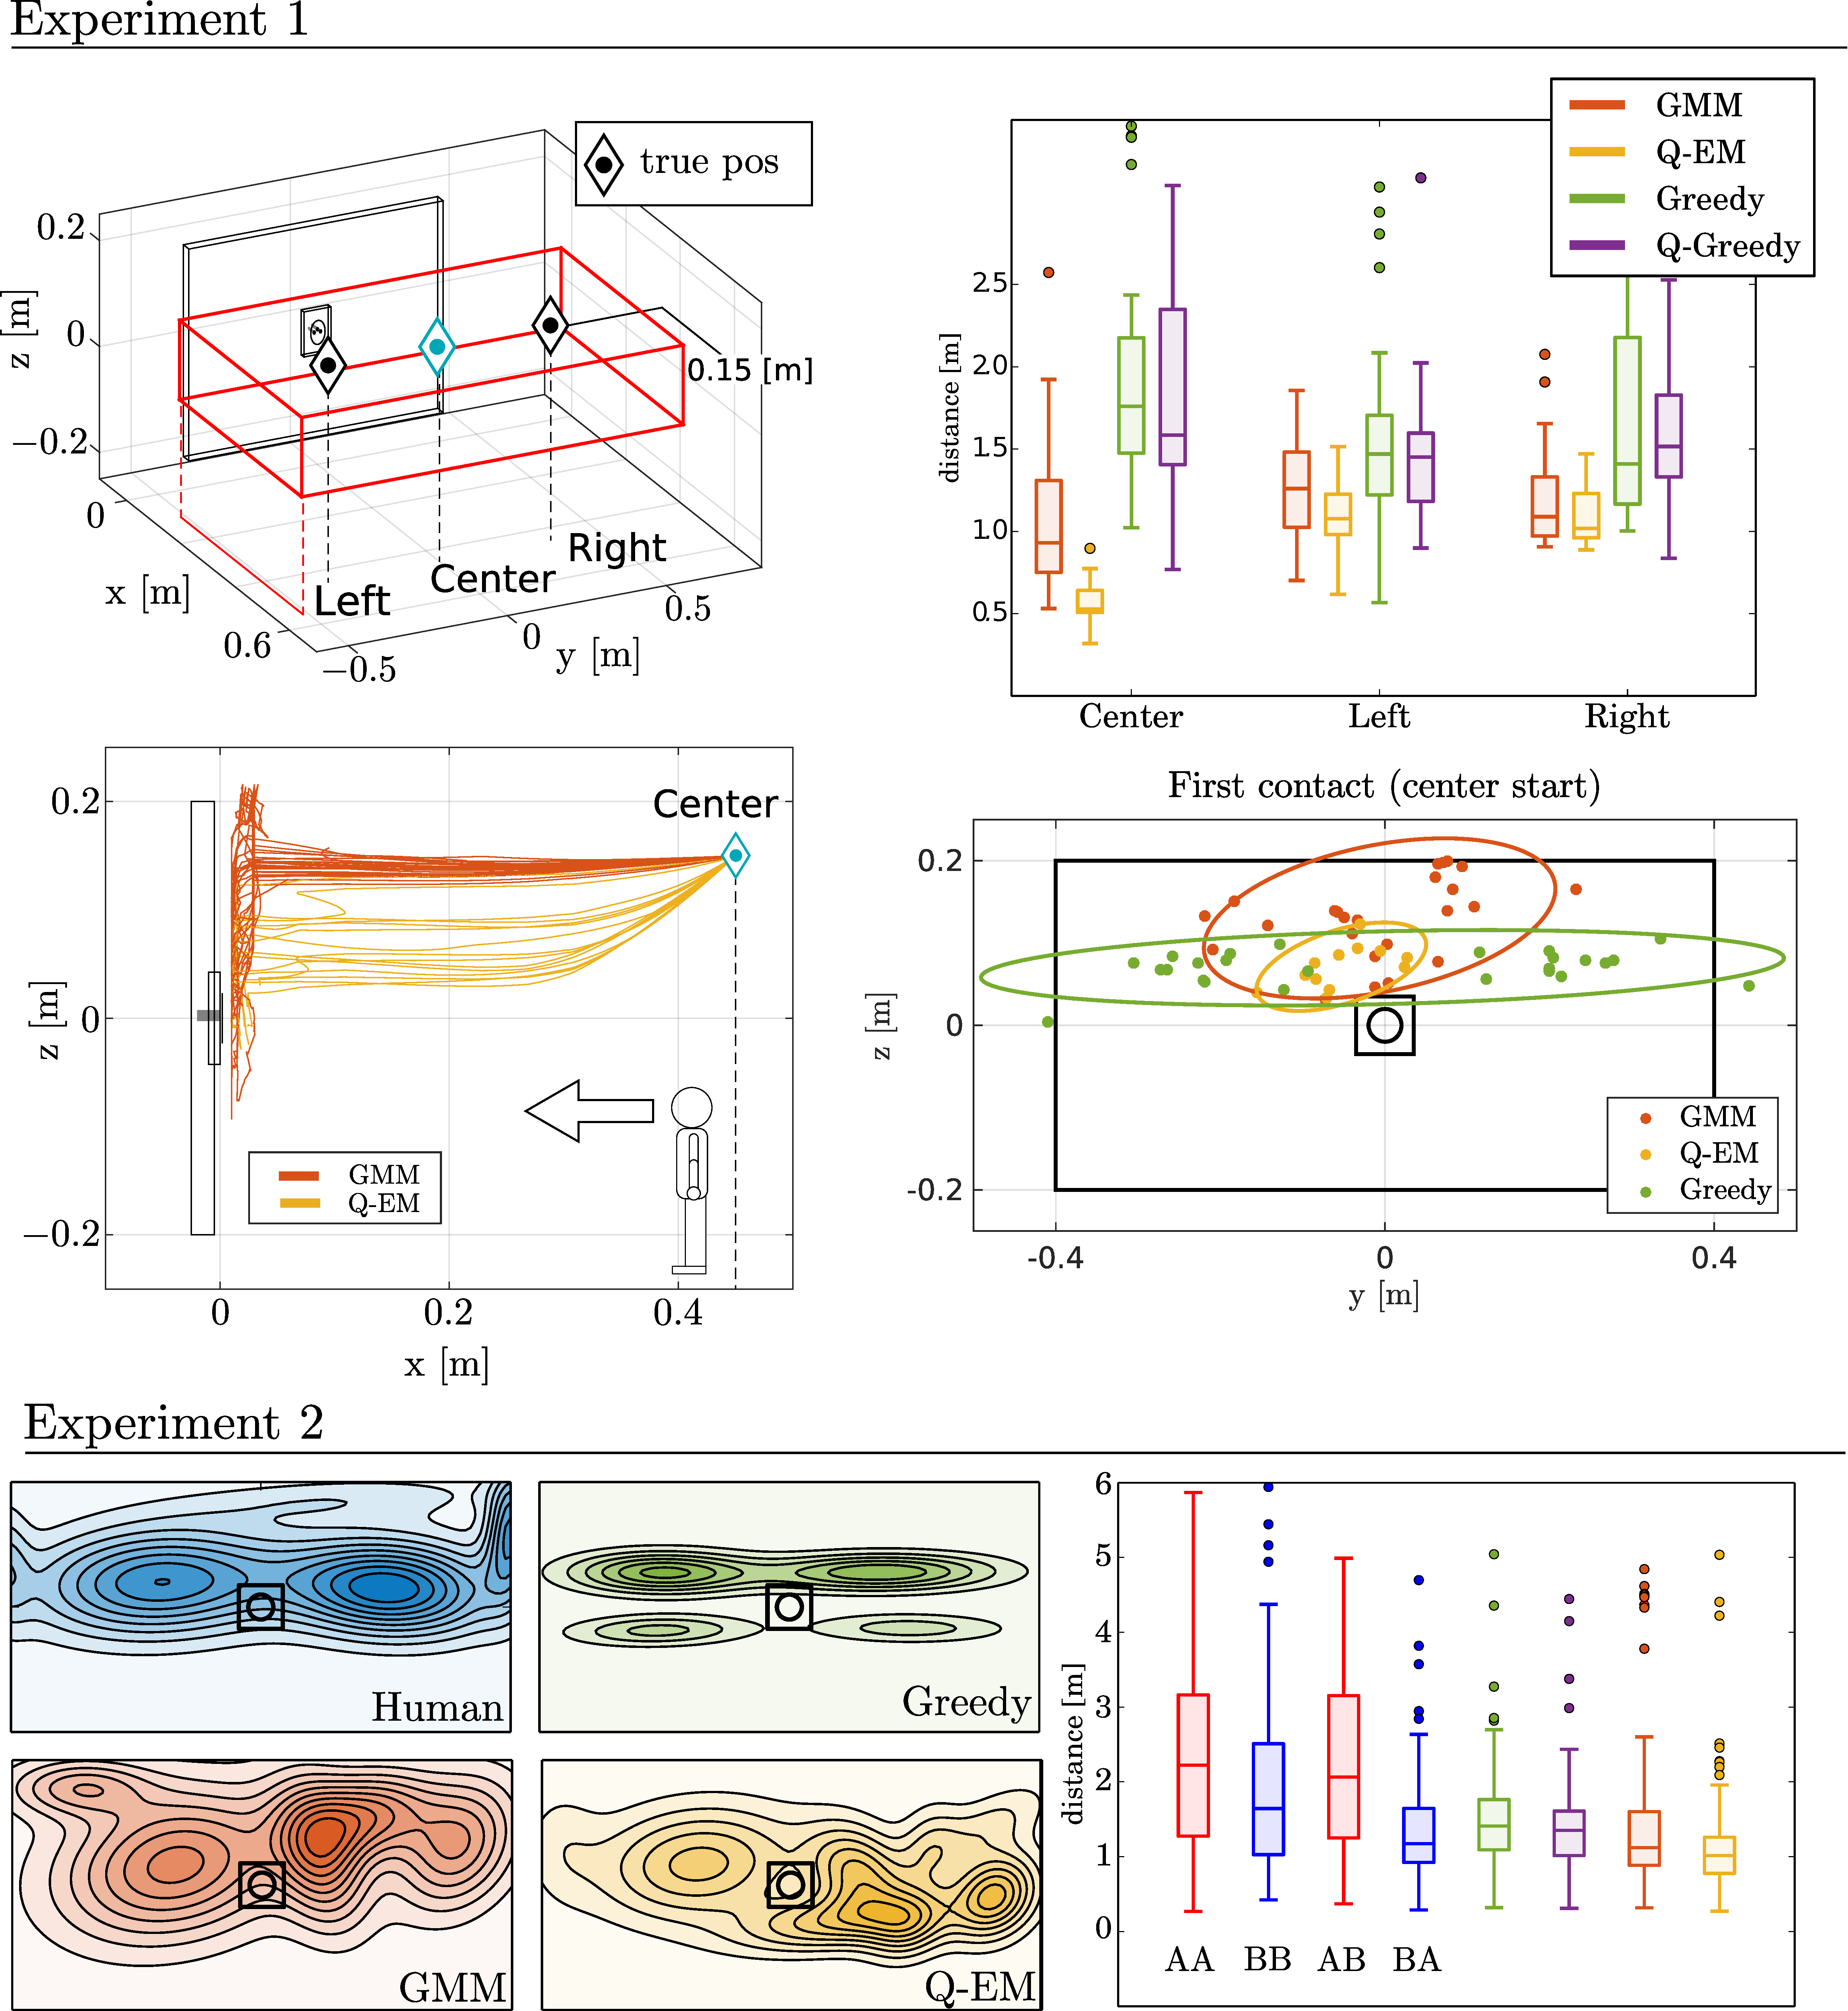
\includegraphics[width=\linewidth]{./Figure/experiment1.pdf}
    \caption{Two simulated search experiments. \textbf{Experiment 1:} \textit{Top-left}: 
     Three start positions are considered: \textit{Left}, \textit{Center} and \textit{Right} in which the triangles depict true position of the end-effector. 
     The red cube illustrates the extent of the uncertainty. \textit{Bottom-left}: Trajectories of both the GMM (orange) and Q-EM (yellow) policies. 
     For each start condition a total of 25 searches were performed for each search policy.
     \textit{Bottom-right:} Distribution of first contact point giving the center initial starting condition. \textit{Top-right}: Distribution of distance 
     travelled until the socket's edge was localised. The Q-EM policy is always the best.
     \textbf{Experiment 2}: \textit{Left}: Distribution of the visited regions during the search for the socket's edge. The Q-EM policy's distribution 
     is more centred along the axis $z=0$. \textit{Right:} Time taken to find the socket, the search algorithms are better than the humans with the exception 
     of group BA.} 
    \label{fig:experiment12}
\end{figure*}

We have shown that under three different experimental settings the Q-EM algorithm is predominantly the best in terms of distance taken 
to localise the socket. The GMM policy learned solely from the data provided by the human teachers also performs well in comparison
with the human teachers and Greedy policy. A critical assumption was made however in order to be able to use this statistical policy approach. 
This \textbf{assumption} is that a human teacher is proficient in accomplishing the task. If a teacher is not able to accomplish 
the task in a repetitive and consistent way so that a search patter can be encoded by the GMM, the learned policy will perform poorly.
Next we evaluate the validity of this assumption and the importance of the training data provided by the human teachers.
 
\subsection{Importance of data}

Two tests were performed to evaluate the importance of the teachers training data, referred to as \textbf{Experiment 3}.
The worst two teachers in terms of distance taken to find the socket's edge are used to learn a GMM and Q-EM policy separately, 
to evaluate whether it is possible to learn a successful policy given a few bad demonstrations 
(15 training trajectories for each policy). In the second test a noisy explorative Greedy policy was used
as a teacher to gather demonstrations which in turn were then used to learn a new policy, which we call Q-Greedy. 

Figure \ref{fig:experiment3} (\textit{Top-left}) illustrates 6 trajectories of teacher \# 5. Once localised, the teacher 
would reposition himself in front of the socket and to try to achieve an insertion. This behaviour was not expected 
since by losing contact with the wall, the human teacher no longer has the sensory feedback necessary 
to maintain an accurate position estimate.

\begin{figure*}
 \centering
    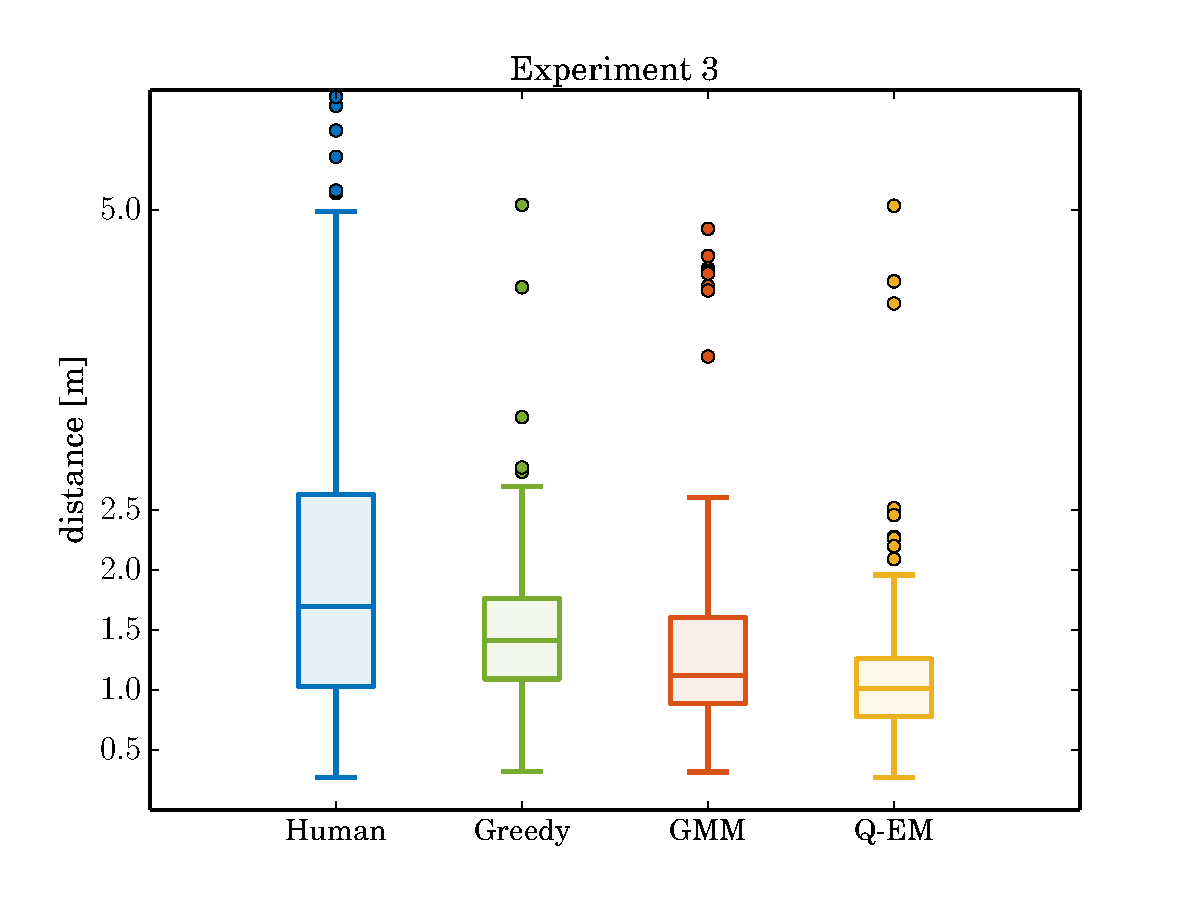
\includegraphics[width=\linewidth]{./Figure/experiment3.pdf}
    \caption{\textbf{Experiment 3} \textit{Top-left}: Demonstrations of teacher \# 5. \textit{Bottom-left} Value function learned from the 15 demonstrations of teacher \#5. The value of the most 
    likely state is plotted. \textit{Middle-column}: Most likely state parameters of the GMM and Q-EM learned from the 
    demonstrations of teacher \#5. \textit{Right-column}: Rollouts of the policies learned from teacher \#5. We can see that trajectories 
    from the GMM policy have not really encoded a specific search pattern, whilst the Q-EM policy gives many more consistent trajectories 
    replicating to some extent the pattern of making a jump (no contact with the wall) from the top right corner to the socket's edge.}
    \label{fig:experiment3}
 \end{figure*}
 
Figure \ref{fig:experiment3} (\textit{Bottom-left}) illustrates the value function of the belief state learned from the data of teacher \# 5.
The states with the highest value seem to create a path going from the socket towards the right edge of the wall. 
As before, to learn a GMM policy is learned from the raw data to produce a Q-EM policy in which the data points are weighted by 
the gradient of the value function. \textit{Experiment 3 Middle-column} illustrates the 
resulting Marginalised Gaussian Mixture parameters for both the GMM and Q-EM policies where 25 rollouts are plotted of each policy starting at 
the \textit{Center} initial condition also used in Experiment 1. It can be seen that the trajectories of the GMM 
policy have much greater variance in contrast to the Q-EM policy, resulting from an excess of variance in the 15 original demonstrations
given by the teacher. Too much variance is not necessarily good, a random (uniform) policy in terms of generated trajectories
will have the most variance and is as expected extremely inefficient in achieving a goal. Furthermore there is insufficient data to encode a pattern for the GMM model. In contrast, the Q-EM finds a 
pattern by combining multiple parts of the available data and as a result fewer data points are necessary to achieve a good policy. 
This effect is clear in Figure \ref{fig:experiment3_stats}, showing the performance of the GMM and Q-EM algorithms 
under the same initial conditions as in Experiment 1. For all the conditions and for both teachers \#5 and \#7 the Q-EM policy 
always does better than the GMM.

\begin{figure}
 \centering
 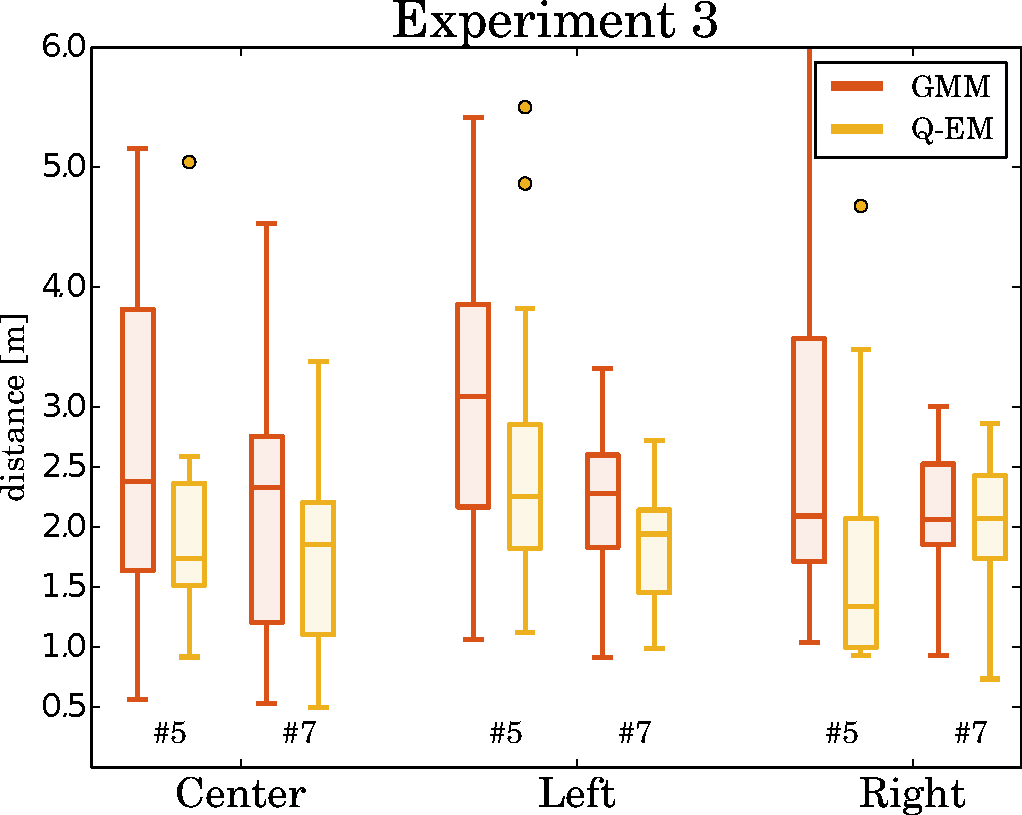
\includegraphics[width=\linewidth]{./Figure/experiment3_stats.pdf}
 \caption{Distance taken to reach the goal for the GMM and Q-EM policies when trained with the 
 worst two teachers. The initial starting conditions are as in Experiment 1. 
 The Q-EM policy nearly always does much better than the GMM policy for both when trained with data 
 from subject \#5 or \#7.}
 \label{fig:experiment3_stats}
\end{figure}

We also tested whether we could use the Greedy policy as a means of gathering demonstrations in order to learn a value function and 
train a Q-Greedy policy. The Q-Greedy policy was used in combination with random perturbations applied to the velocity to act as 
a simple exploration technique. A maximum of 150 searches were performed, which terminated once the socket was found. 
These demonstrations were used to learn a value function and GMM policy which we refer to as Q-Greedy. 
Figure \ref{fig:experiment12} \textit{Experiment 1-2 (bar plot)}, illustrates the statistical results of the 
Q-Greedy policy for Experiment 1 and 2 (purple bar chart), showing that there is no difference between the two policies. 
This exploration method is probably too simplistic to discover meaningful search patterns and we could probably devise better 
search strategies which would result in a better policy. However this study has shown that human behaviour already does have a usable trade-off 
between exploration and exploitation which can be used to learn a new policy through our Fitted Policy Iteration framework.

\subsection{Generalisation}

So far we have trained and evaluated our policies within the same environment.
To test whether the GMM and Q-EM policies can generalise to a new setting the socket
was moved to the upper right corner of the wall. The GMMs were trained in the frame of reference of the socket and
when we translated the socket's location it also translated the policy. 

\begin{figure*}
 \centering
    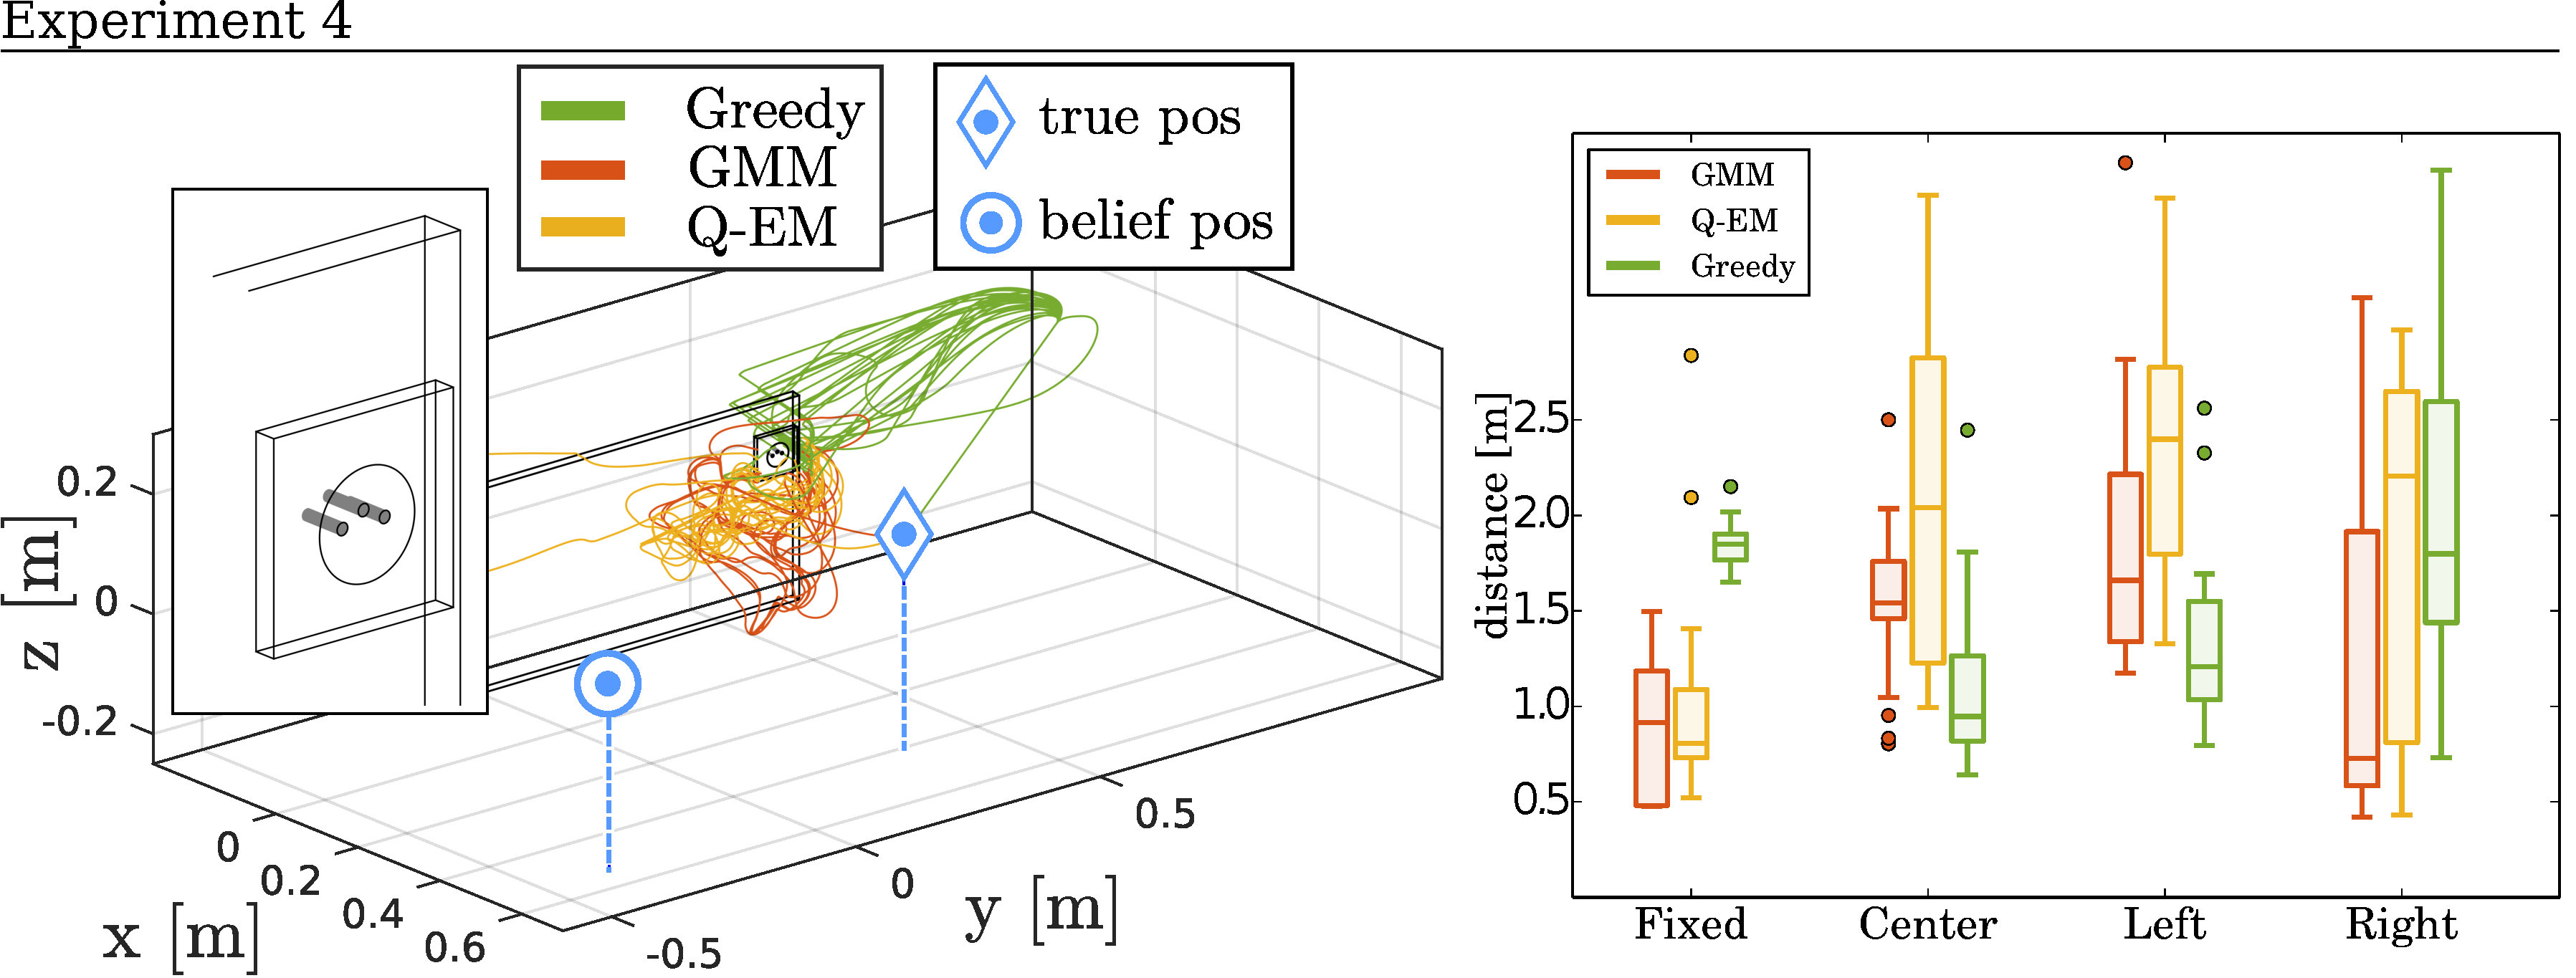
\includegraphics[width=\linewidth]{./Figure/experiment4.pdf}
    \caption{\textbf{Experiment 4} Evaluation of generalisation. The socket is located at the top right corner of the wall. We consider a 
    \textit{Fixed} starting location for both the true and believed locations (most likely state $\hat{x}_t$) of the end-effector. The red square depicted 
    in Figure \ref{fig:experiment12} is the extent of the initial uniform uncertainty. \textit{Right:} Distance taken to reach the socket's edge for 
    four initial starting conditions, left, centre and right of Experiment 1 and the fourth is the fixed condition as previously described. 
    For the Fixed setup both the Q-EM and GMM significantly outperform the Greedy.}
    \label{fig:experiment4}
\end{figure*}


The same initial conditions of Experiment 1 were used with an additional 
new configuration named \textit{Fixed}, in which both the true and believed location are fixed, blue triangle and circle.
Figure \ref{fig:experiment4} \textit{(Left)} illustrates the trajectories of the three search policies for the \textit{Fixed} initial condition. 
The Greedy policy moves in a straight line towards the top
right corner of the table. As the true position is to the right, it takes the Greedy policy longer to find the wall 
in contrast with both the GMM and Q-EM policies. From the statistical results shown in Figure \ref{fig:experiment4} \textit{(Right)} we can see
that for the \textit{Fixed} and \textit{Right} initial condition, which are similar, both GMM and Q-EM are better. However, for 
the \textit{Center} and \textit{Left} initial condition this is no longer the case. 
The Greedy method is better under this condition since the socket is close to informative features (it is located close to the edges of the wall). 
Once the end-effector has entered in contact with the wall the actions of the Greedy policy always result in a decrease of uncertainty, which was not the case when the socket was located in the center of wall. 
Thus in both the \textit{Fixed} and \textit{Right} initial condition the Greedy method does worse because it takes longer
to find the wall.

The GMM based policies are still able to generalise under different socket locations. In general, as the socket's location is moved 
further from the original frame of reference in which it was learned, the higher is the likelihood that the search quality degrades. We 
chose the upper right corner since it is the furthest point from the origin and the GMM and Q-EM policies were still able to find 
the socket. We note that the policy will always be able to find the socket once it has localised itself. This can be seen from the vector field 
of the GMM policy when the uncertainty is low, see Figure \ref{fig:policy_vf} on page \pageref{fig:policy_vf}. In this case the policy is a sink function 
with a single point attractor.

% Real socket experiment.

\subsection{Distance taken to connect the plug to the socket}

This section evaluates the distance taken for the policies and humans to establish a connection, after the socket 
has been found. The distance is measured from the point that the plug enters in contact with the socket's edge until 
the plug is connected to the socket. All the following evaluations are done on a KUKA LWR4 robot. The robot's end-effector 
is equipped with a plug holder on which is attached a force-torque sensor, the same holders used during the 
human teachers' demonstrations. In this way both the teacher and robot apprentice share the same sensory interface.

We chose to have the robot's end-effector located to the right of the socket and a belief spread uniformly 
along the z-axis. See Figure \ref{fig:real_pictures} for an illustration of the initial starting condition.
This initial configuration was used to evaluate the search policies for the three different sockets, see Figure \ref{fig:search_task_setup} 
on page \pageref{fig:search_task_setup} for an illustration of the sockets. The same initial configuration for 
the evaluation of the three sockets was kept in order to observe the generalisation properties of the policies. 
Note that only the training data from demonstrations acquired during the search with socket A were used. 
Socket B has a funnel which should make it easier to connect whilst socket C should be more difficult as it has no informative features on its surface. 

For each of the sockets 25 searches were performed starting from the same initial condition. 
In Figure \ref{fig:real_pictures} \textit{(Left)} we plot the trajectories of each of the search methods for socket A. The GMM reproduces some of the behaviour exhibited by humans, such as 
first localising itself at the top of the socket before trying to attempt to make a connection. The Q-EM algorithm exhibits less variation
than the GMM and tends to pass via the bottom of the socket to establish a connection. The Greedy method in contrast is much more  
stochastic since it does not take into consideration the variance of the uncertainty but instead tries to directly establish a connection.
In Figure \ref{fig:real_pictures} \textit{(Right)} illustrates a typical rollout of the GMM search policy for both 
socket A and C. Once a contact is made with the socket's edge the policy tends to stay close to informative features and tends to 
wander vertically up and down. Only when the uncertainty has been reduced does the GMM policy go towards the socket's connector. 

\begin{figure*}
 \centering
 \includegraphics[width=0.95\textwidth]{./Figure/real_experiment_v2.pdf}
 \caption{\textit{Left}: 25 search trajectories for each of the three search policies for socket A. 
 \textit{Right} KUKA LWR4 equipped with a holder mounted with a ATI 6-axis force-torque sensor. \textit{Socket A}: The robot's end-effector starts to the 
 right of the socket. The second row shows screen captures taken of ROS Rviz data visualiser in which we see the Point Mass Filter 
 (red particles) and a yellow arrow indicating the direction given by the policy. In this particular run, the plug remained in contact with the ring of the socket until 
 the top was reached before making a connection. \textit{Socket C}: Same initial condition as for socket A. The policy leads the plug down to 
 the bottom corner of the socket before going the center of the top edge, localising itself, and then making a connection. See \href{http://lasa.epfl.ch/videos/gpldecha/pih-search/KUKA_socket_B_connection.wmv}{Video 4}
 and \href{http://lasa.epfl.ch/videos/gpldecha/pih-search/KUKA_socket_C_connection.wmv}{Video 5} for an illustration of the KUKA establishing a connection to socket B and C.
 }
 \label{fig:real_pictures}
\end{figure*}

The GMM and Q-EM policies are able to generalise to both socket B and C, as the geometric shape and connector interface of the 
two sockets are similar to socket A. The local force modulation of the policy's vector field, which is not learned, allows the 
end-effector to surmount edges and obstacles whilst trying to maintain a constant contact force in the x-axis. 
This modulation makes it possible for the plug to get on top of socket C.

Figure \ref{fig:real_statistics} (a) illustrates the statistics of the distance taken to establish a connection for all three sockets.
For socket A both the Greedy and Q-EM are better than the GMM and the Q-EM has less variance in comparison to the Greedy searches.  
All three search methods are vastly superior, when compared to the human's performance see Figure \ref{fig:real_statistics} (b-c).

The interesting point is that both the GMM and Q-EM algorithms perform better than the Greedy approach for socket C. Socket C has no informative 
features on its surface and as a result myopic policies such as the Greedy policy will perform poorly. However for socket A 
and B, the Greedy policy performs better as both of these sockets have edges around their connector point allowing for easy localisation. 
It can also be seen that most search methods perform better on socket B than A, since the funnel shape connector helps in maintaining the plug 
within the vicinity of the socket's holes. We found that the insertion policy $\pi_{\Param_2}(\omega|\phi)$ only helped with the insertion 
when the wall was artificially rotated such that a direct insertion was not possible. Otherwise the insertion was always successful 100\% of 
the time. In other more industrial applications the insertion step is more problematic than when considering an electric socket, 
see \cite[Chap. 5]{Kronander2015} for further details on the jamming dilemma. 

The discrepancy between the humans performance and the search policies can be attributed to many causes. One plausible reason is 
that the PMF probability density representation of the belief is more accurate than the human teachers' position belief. 
Also, the motion noise parameter was fixed to be proportional to the velocity and the robot moves at gentle pace ($\sim1$ cm/s) as 
opposed to some of the human teachers. In actuality, humans are far less precise than the KUKA which has sub-millimetre accuracy.

\begin{figure*}
 \centering
   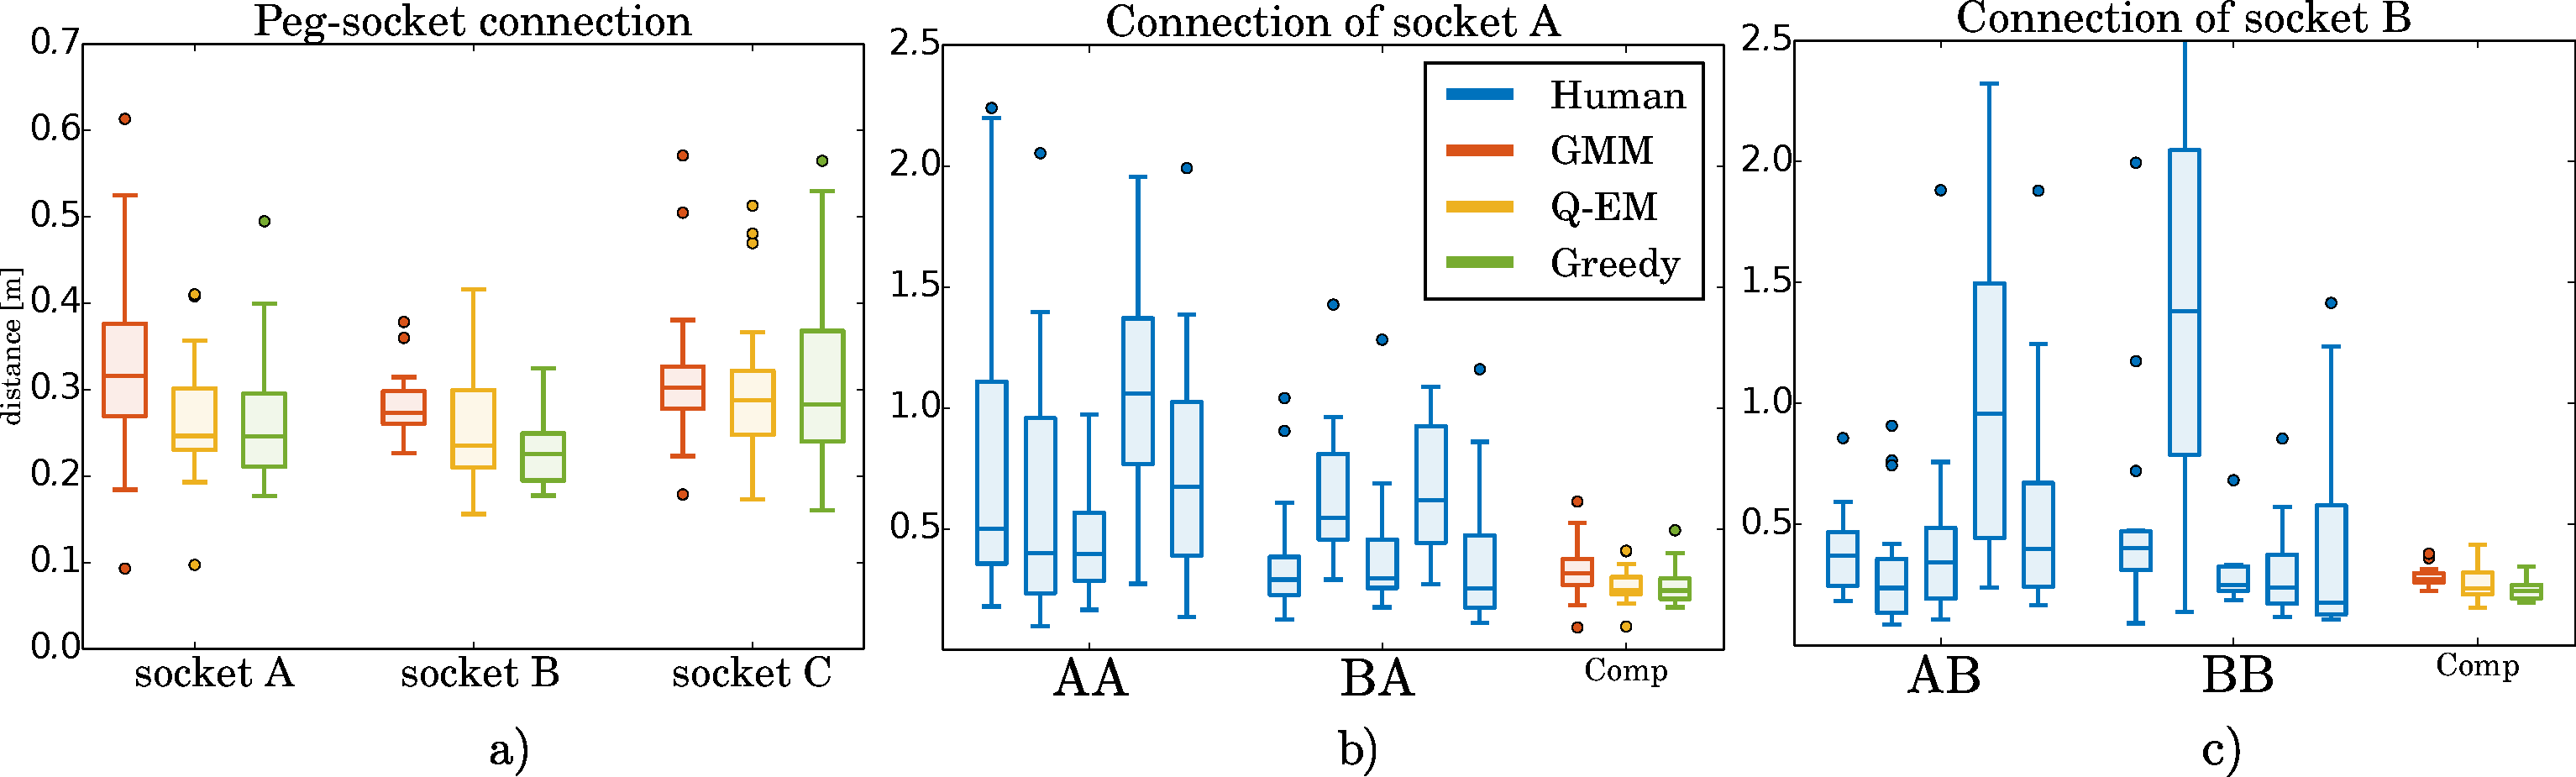
\includegraphics[width=\linewidth]{./Figure/real_socket_human_all.pdf}
  \caption{ Distance taken to connect the plug to the socket (a) The Q-EM algorithm is the best for both socket A and C. 
  For socket C, the Greedy algorithm does worse than the other two. This is because socket C has no informative features. 
  (b) Group AA are the set of teachers who first started with socket A. They had no previous training on another socket beforehand. Group 
  BA first gave demonstrations on Socket B before giving demonstrations on Socket A. Group BA
  is better than Group AA at doing the task. This is most likely a training effect. However all policy search methods are far better
  at connecting the plug to the socket. (c) Both Groups AB and BB are similar in terms   of the distance they took to 
  insert the plug into the socket, the search policies on the other hand travel less to accomplish the task.   } 
  \label{fig:real_statistics}
\end{figure*}


\section{Discussion \& Conclusion}\label{sec:conclusion}
% Recapulate what we did 

In this work we learned search policies from demonstrations provided by human teachers for a task
which consisted of first localising a power socket (either socket A, B or C) and then connecting it with a plug. Only haptic information 
was available as the teachers were blindfolded. We made the assumption that the position belief of the human teachers 
was initially uniformly distributed in a fixed rectangular region of which they were 
informed and is considered prior knowledge. All subsequent beliefs were then updated in a Bayesian recursion 
using the measured velocity obtained from a vision tracking system, and wrench acquired from a force torque sensor attached 
to the plug. The filtered probability density function, represented by a Point Mass Filter, was then compressed to the 
most likely state and entropy.

Two Gaussian Mixture Model policies were learned from the data recorded during the human teachers' demonstrations. 
The first policy, called Q-EM, was learned in an Actor-Critic RL framework in which a value function was learned over 
the belief space. This was then used to weight training datapoints in the M-step update of Expectation-Maximisation (EM). The second 
policy, called GMM, was learned using the standard EM algorithm, and considered all training data points equally,
following in the footsteps of our initial approach \cite{Chambrier2014}. Both the Q-EM and GMM policies were trained 
with data solely from the human demonstrations of the search with socket A.

Four different aspects of the learned policies have been evaluated. Firstly, which of three policies, Q-EM, GMM and a Greedy policy, 
took the least distance to find the socket. Across three different experiments it was shown that the Q-EM algorithm always performs
the best. It was clear that the Q-EM policy was less random and more consistent than the GMM policy as it tried to enter in 
contact with the wall at the same height as the socket thus increasing the chances of finding the socket.

Secondly, the importance of the data provided by the human teachers was tested. The data from the two worst teachers was used to 
train an individual GMM and Q-EM policy for each of them. It was found that the performance of the Q-EM was better than the GMM in terms 
of distance travelled to find the socket. When qualitatively evaluating the trajectories of the GMM with respect to the 
Q-EM for the worst teacher, it is clear that the Q-EM policy managed to extract a search pattern, which was not the case 
for the GMM policy. A Q-EM policy was also learned from the data provided by a Greedy policy with explorative noise 
and no improvement was found. From these results we conclude that the exploration and exploitation aspects of the trajectories 
provided by the human teachers is necessary.

Thirdly, the two policies (GMM and Q-EM) were tested to see whether they were able to generalise to a different socket location. 
Under a specific condition, called \textit{Fixed}, both policies were significantly better than the Greedy policy. However for the \textit{Center}
and \textit{Left} initial conditions the Greedy policy performed better. When the Greedy policy 
enters in contact with the wall at an early stage, it performs better than the GMM and Q-EM. The reason for this is that  
the actions taken by the Greedy policy in this setting will always result in a decrease of entropy when the location
of the socket is close to a corner, as opposed to being in the center of the wall.

Fourthly, all three policies were evaluted on the KUKA LWR robot and all performed better than the human 
teachers. For socket A there is no clear distinction between 
the Q-EM and Greedy policy. On socket B, which was novel, the Greedy policy performed better than the statistical controllers, 
which we hypothesize was a result of a funnel which would make it easier for a myopic policy. For socket C, both the 
GMM and Q-EM policies performed better than the Greedy, as socket C has no features on its surface, this being a disadvantage 
for a myopic policy.

We conclude that by simply adding a binary reward function in combination with 
data provided by human demonstrations, using fitted reinforcement learning, better policy can be learned without 
the need to perform expensive exploration-exploitation rollouts traditionally associated with reinforcement learning and 
designing complicated reward functions. This is especially advantageous when only a few demonstrations are available.


\FloatBarrier
\bibliographystyle{elsarticle-harv} 
\bibliography{bib/ras_fpi.bib}

\end{document}

\endinput
